% Description: 	Template for U-SPACE CDR documentation
% Authors:		Morten Olsen & Dries Agten

% HOW TO USE THIS TEMPLATE?
%
% 1. Open and edit the following files: 
%		- introduction.tex
%		- requirements.tex
%		- mse.tex
%		- eps.tex
%		- mcc.tex
%		- itpu.tex
%		- thermal_pyro_emc.tex
%		- test_verification.tex
%		- ground_support.tex
%		- project_management.tex
%
% 2. Compile the report from this file (TEMPLATE.tex), using the following sequence:
%		a. PDFLaTex
%		b. BibTex
%		c. PDFLaTex
%		d. PDFLaTex
% 
% 3. Rename the output pdf-file, according to the document reference number (line 89 in this file)
%
% 4. Enjoy the outcome! :-)
%
% If you experience problems, try to search on Google or contact Morten Olsen or Dries Agten
%
\documentclass[a4paper,11pt,titlepage]{report}
\usepackage[english]{babel}
\usepackage[margin=3cm]{geometry}
\usepackage[T1]{fontenc}
\usepackage[utf8]{inputenc}
\usepackage{lmodern}
\usepackage[sorting=none]{biblatex}
\usepackage{graphicx}
\usepackage{fancyhdr}
\usepackage[textfont={small,it},labelfont=bf,labelsep=endash]{caption}
\usepackage[table]{xcolor}
\usepackage{verbatim}
\usepackage[toc,page]{appendix}
\usepackage{url}
\usepackage{amsmath}
\usepackage{multicol}	% allow multi column environemnt
\usepackage{float} % forced position of figures/tables etc.
\usepackage{acronym}
\usepackage{rotating}
\usepackage{titling}
\usepackage{bibcheck}
\usepackage[center]{subfigure} % make it possible to include more than one captioned figure/table in a single float
\usepackage[pdfstartview=FitH,pdfborder={0 0 0},bookmarks]{hyperref}
\usepackage{memhfixc}
\usepackage{placeins}
\usepackage{longtable} % multi-page table environment
\usepackage{tabularx}
%\usepackage[pdftex]{hyperref}
\hypersetup{colorlinks=true, linkcolor=black, citecolor=black, filecolor=black, urlcolor=black,
pdftitle={U-SPACE Critical Design Report}}


\graphicspath{{./figures/}}	% look for graphic files in the "figures" subfolder

\definecolor{tableshade}{HTML}{E8E8E8}
\linespread{1.3}

% define the page headers and footers
\fancyhead{}
\fancyhead[RE,RO]{\parbox[b]{10cm}{\raggedleft U-SPACE\\ \today}}
\fancyhead[LE,LO]{\parbox[b]{10cm}{\docreference \\ \title }}
\renewcommand{\headrulewidth}{0.4pt}
\fancyhfoffset{1cm}
\addtolength{\headheight}{1cm}
\fancyfoot{}
\fancyfoot[C]{\thepage}
\renewcommand{\footrulewidth}{0.4pt}
\newcommand{\rr}{\raggedright} % to use for force left-align in multi-row table cells
\newcommand{\tn}{\tabularnewline} % to use for making the above work :-)

\bibliography{references} % include .bib file for citations

% PLEASE FILL IN THE RELEVANT INFORMATION BELOW:
%
\def\authors{ \vspace{-1.0em}
\begin{tabbing}
Dries \textsc{Agten} \hspace{2.5em} \= Mauro \textsc{Aja Prado} \\
Ishan \textsc{Basyal} \> Pedro \textsc{Cervantes} \\
Bastian \textsc{Hacker} \> Zhou \textsc{Hao} \\
Morten \textsc{Olsen} \> Oliver \textsc{Porges} \\
Jan \textsc{Sommer} \> Anuraj \textsc{Rajendraprakash} \\
Tiago \textsc{Rebelo} \>
Omair \textsc{Sarwar}
\end{tabbing}
}
\def\docversion{RELEASED}					% Possible versions are: DRAFT, REVIEW or RELEASED
\def\docreference{USPACE-CDR-A2}	% -00 = DRAFT,  -A1 = 1st release,  -A2 = 1st release with minor updates, -B1, = 2nd release
\def\title{Critical Design Report}


\begin{document}

\begin{titlepage}

\begin{center}


\includegraphics[width=0.6\textwidth]{figures/logo.pdf}\\[0.75cm] 

\textsc{\large Unmanned Solar Powered Airship Concept Evaluation}\\[1cm]

\line(1,0){415}\\[1mm]
\vspace{-1.0em}
\Huge \bfseries{\title}\\[2mm] 
%\
\vspace{-1.0em}
\line(1,0){415}\\[1cm]

\begin{large}
\begin{tabular}{ll}
Document Reference No.: & \docreference\\[5mm]
Document Status: & \docversion \\[1.5cm]
\end{tabular}
\end{large}

\begin{minipage}[t]{0.49\textwidth}
\begin{flushleft} \large
\emph{Authors}\\
\vspace{-1.2em}
\line(1,0){125}\\
\footnotesize{\authors}
\end{flushleft}
\end{minipage}
\begin{minipage}[t]{0.49\textwidth}
\begin{flushright} \large
\emph{Supervisors}\\
\vspace{-1.2em}
\line(1,0){125}\\
Kjell \textsc{Lundin}\\
Alf \textsc{Wikstr\"{o}m}
\end{flushright}
\end{minipage}

\vspace{1cm}

\begin{minipage}[t]{0.49\textwidth}
\begin{flushleft} \large
\emph{Project Manager}\\
\vspace{-1.2em}
\line(1,0){125}\\
Dries \textsc{Agten}
\end{flushleft}
\end{minipage}
\begin{minipage}[t]{0.49\textwidth}
\begin{flushright} \large
\emph{Quality Manager}\\
\vspace{-1.2em}
\line(1,0){125}\\
Morten \textsc{Olsen}\\[1cm]
\end{flushright}
\end{minipage}

\vfill

\begin{large}
\today \\
Lule\r{a} University of Technology \\
Rymdcampus, Kiruna, Sweden\\
\end{large}

\end{center}

\end{titlepage}

\pagestyle{plain}
\pagenumbering{roman}

\thispagestyle{plain}
\chapter*{Normative References}
\markboth{Normative References}{Normative References}
\addcontentsline{toc}{chapter}{\protect\numberline{}Normative References}
%
\begin{table}[H]
\centering
\caption{Normative References for this document}
\label{tab:normative_references}
\begin{tabular}{lll}
\hline
\textbf{Document title} & \textbf{Doc. Ref. No.} & \textbf{Doc. status}\\
\hline
Critical Design Report & USPACE-CDR-A2 & Released\\
\hline
\end{tabular}
\end{table}
%
\newpage
%
\thispagestyle{plain}
\chapter*{Document Change Record}
\markboth{Document Change Record}{Document Change Record}
\addcontentsline{toc}{chapter}{\protect\numberline{}Document Change Record}
%
%
\begin{table}[H]
\centering
\caption{Document Change Record for this document}
\label{tab:document_change_record}
\begin{tabular}{p{0.22\textwidth}p{0.25\textwidth}p{0.42\textwidth}}
\hline
\textbf{Doc. version} & \textbf{Change date} & \textbf{Change Description}\\
\hline
USPACE-FR-A1 & \today & 1st release\\
\hline
\end{tabular}
\end{table}
\thispagestyle{plain}
\chapter*{Acronyms}
\markboth{Acronyms}{Acronyms}
\addcontentsline{toc}{chapter}{\protect\numberline{}Acronyms}

\begin{multicols}{2}
\begin{acronym}
\acro{ADCS}{Attitude determination and control}
\acro{ADC}{Analog to Digital converter}
\acro{ADS}{Attitude Determination System}
\acro{BCR}{Battery Charge Regulator}
%\acro{BJT}{Bipolar Junction Transistor}
%\acro{CC}{Constant Current}
\acro{CDR}{Critical Design Review}
%\acro{CM}{Current Mode}
\acro{COTS}{Commercial Off-The-Shelf}
\acro{CPU}{Central Processing Unit}
\acro{CRC}{Cyclic Redundancy Check}
%\acro{DCM}{Discontinuous Conduction Mode}
\acro{DM}{Development Model}
\acro{DSP}{Digital Signal Processor}
\acro{ECSS}{European Cooperation for Space Standardization}
\acro{EGSE}{Electrical Ground Support Equipment}
\acro{EKF}{Extended Kalman Filter}
\acro{EMC}{Electromagnetic Compatibility}
\acro{EMI}{Electromagnetic Interference}
\acro{EPS}{Electrical Power System}
\acro{ESC}{Electronic Speed Control}
%\acro{ESR}{Equivalent Series Resistor}
\acro{ETSI}{European Telecommunications Standards Institute}
\acro{FM}{Flight Model}
%\acro{FRR}{Flight Readiness Review}
\acro{GPS}{Global Positioning System}
\acro{$I^2C$}{Inter-Integrated Circuit}
\acro{IC}{Integrated Circuit}
%\acro{IDC}{Insulation Displacment Connector}
\acro{IRF}{Swedish Institute of Space Physics}
\acro{ISE}{Integrated software environment}
\acro{ITPU}{Imaging and Tracking Payload Unit}
\acro{ITU}{International Telecommunication Union}
\acro{LDO}{Low-dropout}
\acro{LiPo}{Lithium-Polymer}
\acro{LTU}{Lule\r{a} University of Technology}
\acro{MCC}{Motor Control and Communication}
\acro{MCU}{Micro-Controller Unit}
%\acro{MEA}{Main Error Amplifier}
\acro{MGSE}{Mechanical Ground Support Equipment}
%\acro{MOSFET}{Metal-Oxide-Semiconductor Field-Effect Transistor}
%\acro{MPP}{Maximum Power Point}
\acro{MPPT}{Maximum Power Point Tracking}
%\acro{MPPTU}{Maximum Power Point Tracking Unit}
\acro{MSE}{Mechanical Structure and Envelope}
%\acro{NTC}{Negative Temperature Coefficient}
\acro{OBDH}{Onboard Data Handling}
%\acro{OpAmp}{Operational Amplifier}
\acro{OSI}{Open Systems Interconnection}
\acro{PCB}{Printed Circuit Board}
\acro{PDR}{Preliminary Design Review}
%\acro{SA}{Solar Array}
%\acro{PSA}{Pressure Sensitive Adhesive}
%\acro{PTC}{Positive Temperature Coefficient}
\acro{PWM}{Pulse Width Modulation}
%\acro{RHPZ}{Right Half Plane Zero}
\acro{RMP}{Rounds Per Minute}
\acro{SAR}{Solar Array Regulator}
\acro{SD}{Secure Digital}
\acro{SMD}{Surface-Mount Device}
\acro{SoC}{System on Chip}
\acro{SPA}{Solar Powered Airship}
\acro{SSC}{Swedish Space Corporation}
\acro{TBD}{To Be Decided}
\acro{U-SPACE}{Unmanned Solar Powered Airship Concept Evaluation}
\acro{UART}{Universal Asynchronous Receiver/Transmitter}
%\acro{UAS}{Unmanned Aircraft System}
%\acro{UAV}{Unmanned Aerial Vehicle}
\acro{USB}{Universal Serial Bus}
\acro{UVLO}{Under-Voltage Lock-Out}
\acro{TTC}{Telemetry, Tracking and command}
\acro{ISM}{Industrial, Scientific and Medical}
\acro{RF}{Radio Frequency}
\acro{TC}{Telecommand}
\acro{TM}{Telemetry}
\acro{URL}{Uniform Resource Locator}
\end{acronym}
\end{multicols}

\markboth{List of Figures}{List of Figures}
\addcontentsline{toc}{chapter}{\protect\numberline{}List of Figures}
\listoffigures
\newpage

\markboth{List of Tables}{List of Tables}
\addcontentsline{toc}{chapter}{\protect\numberline{}List of Tables}
\listoftables
\newpage

\tableofcontents
\newpage
\acresetall	%reset acronyms which is otherwise used in list of figures or tables
\clearpage %reset page numbers
\pagenumbering{arabic}
\pagestyle{fancy}

\newpage
\section{Introduction}
\label{sec:introduction}

The \ac{EPS} provides power to motors, the on-board computer, communication system and payloads. Power is mainly supplied from solar cells but can also be supplied from a battery, when solar power is not available or insufficient. 

\subsection{Changes from PDR to CDR}
\label{sec:changes_pdr_to_cdr}
%
Table \ref{tab:pdr_to_cdr} lists major design changes from the \ac{EPS} \ac{PDR} report.

\begin{table}[H]
\centering
\caption{U-SPACE \ac{EPS} design changes from PDR to CDR}
\label{tab:pdr_to_cdr}
\begin{tabular}{p{0.25\textwidth}p{0.2\textwidth}p{0.45\textwidth}}
\hline
\textbf{Area of change} & \textbf{Changed parameter } & \textbf{Argumentation for change}\\
\hline
Total power budget & Increased to $>40\,W$ & Airship total mass and size are increased thus requiring much more power for the motors\\
Solar cells & New part & Old solar cell was much heavier than listed in manufacturer datasheet due to a glass cover\\
Total system cost & Increased to $>12000\,SEK$ & Increased power and new light-weight solar cells are more expensive\\
Solar cell mounting & New part & New solar cell is flexible instead of rigid and can be mounted with \ac{PSA}\\
\hline
\end{tabular}
\end{table} 
\chapter{Goals and Constraints}
\label{chap:goals_constraints}

\section{Project Goals}
\label{sec:goals}
%What function(s) does the subsystem have to fulfill?

The principal goal of the \ac{U-SPACE} project is to try and bridge the gap between a student-driven engineering project and the concept of an unmanned \ac{SPA}. As very few examples of this type of design exist \cite{website:solr}, much is to be gained from this project. Due to the many constraints that have to been taken into account (see section \ref{sec:constraints}), the goal is necessarily modest. The goal of this project is thus designing, building and testing a small-scale \ac{SPA} for low altitude flight, including support for a scientific payload. The basic targets are listed below:

\begin{itemize}
\item Design of a small unmanned \ac{SPA} capable of forward propulsion, powered by solar cells and including a scientific payload
\item Construction of such an \ac{SPA} with minimal cost
\item Flight test of this \ac{SPA} at low altitude
\end{itemize}

\section{Project Constraints}
\label{sec:constraints}
%What technical requirements constrain the subsystem design? - e.g. mass, power, strength, stability etc.

The design, construction and test of a small unmanned \ac{SPA} is susceptible to many constraints, all of which have to be identified, examined and finally dealt with. These constraints take many forms, but may be divided into four categories: functionality, resources, environment and law.

\subsection{Functionality}

The \ac{U-SPACE} project, being a proof of concept, consists of designing, building and testing a small version of a \ac{SPA} with a limited scientific payload. Therefore reasonable limits have to be taken into account for some technical parameters. These parameters and their limits are listed below in table \ref{tab:functionality}.

\begin{table}[H]
\centering
\caption{Functional parameters and limits}
\label{tab:functionality}
\begin{tabular}{c c c}
\hline
\textbf{Parameter} & \textbf{Lower limit} & \textbf{Upper limit}\\ \hline
Total mass & / & 4.5 kg\\
Flight altitude & 2 m & 100 m\\
Electrical power & / & 40 W\\
Forward velocity & / & 1 m/s\\
Radius & 10 m & /\\
\hline
\end{tabular}
\end{table}

\subsection{Resources}

Since the \ac{U-SPACE} project is a student project supported by \ac{LTU} and \ac{IRF}, the available resources are limited. This imposes stringent constraints on all phases of the project. The main resources can be identified as the three elements of the project management triangle, shown in figure \ref{fig:project_triangle}.

\begin{figure}[htbp!]
\centering
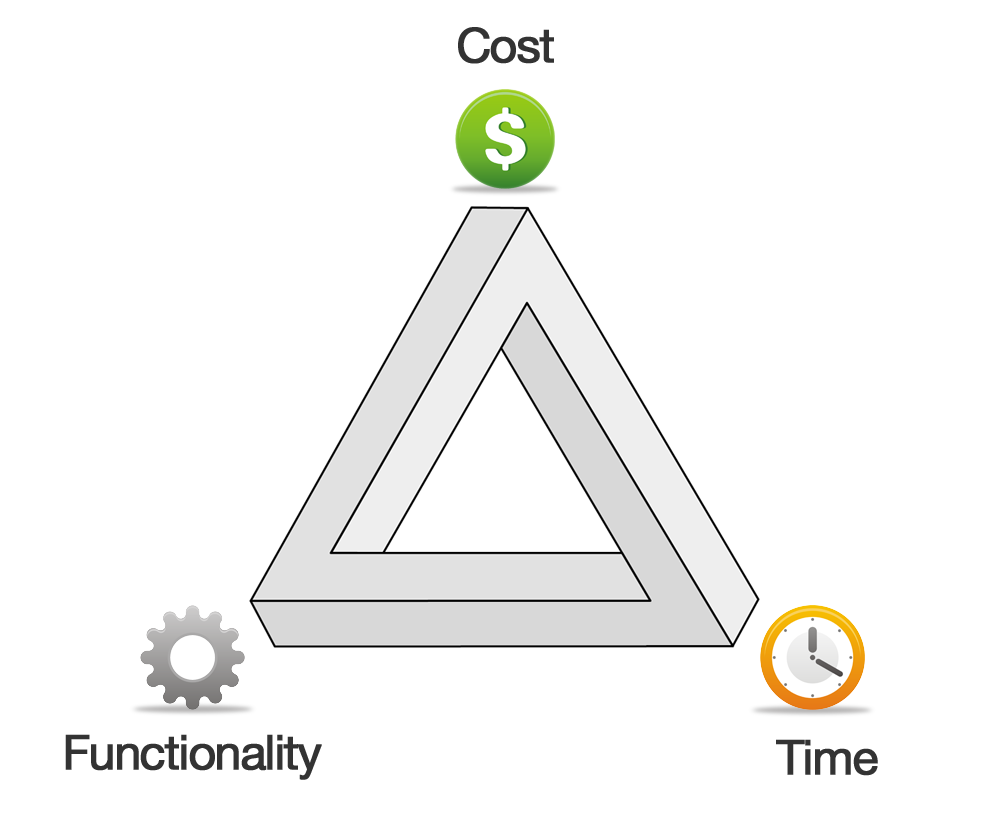
\includegraphics[scale=0.2]{figures/project_triangle.png}
\caption[Project management triangle]{Project management triangle \cite{website:claromentis}.}
\label{fig:project_triangle}
\end{figure}

\noindent
The cost of this student project is limited by its approved budget, a sum between 10,000 and 12,500 SEK, provided by \ac{LTU}. More funding can be applied for if required, but the budget nevertheless remains limited. This constraint implies a careful selection of components and the use of innovative engineering solutions throughout the entire project. 
\\
\\
The time available for this project is also constrained, being a student project that has to be realized in concurrence with other academic duties. The estimated time frame is therefore between 2 and 6 months for a first prototype capable of test flight.
\\
\\
The final resource is related to the previously mentioned functionality. With a limited number of team members that have limited expertise in the field of airships, the project has to be technically balanced, taking into account the capabilities of the members of the team.

\subsection{Environment}

The \ac{SPA} that will be developed during the \ac{U-SPACE} project finally has to be tested outdoors. Since the \ac{U-SPACE} project is being executed in the city of Kiruna during the spring, summer and early autumn, it is important to take the environmental conditions during this period of the year into account.  Some of the these conditions are listed below in table \ref{tab:environment}, using data for the month of May \cite{website:weatherspark} as a representation of the entire project period.

\begin{table}[H]
\centering
\caption{Environmental conditions}
\label{tab:environment}
\begin{tabular}{p{0.35\textwidth} p{0.15\textwidth} p{0.15\textwidth} p{0.35\textwidth}}
\hline
\textbf{Parameter} & \textbf{Lower boundary} & \textbf{Upper boundary} & \textbf{Remarks}\\ \hline
Temperature & -2 $^\circ$C & 11 $^\circ$C & Average values\\
Wind speed & 1 m/s & 6 m/s & Usually from the south west\\
Probability of precipitation & 61 \% & 61 \% & Average value\\
Hours of sunshine & 17:38 h & 22:45 h & Daily values\\
Cloud cover & 83 \% & 83 \% & Median value\\
Solar incidence angle at noon & 46 $^\circ$ & 46 $^\circ$ & Refer to document USPACE-PDR-PWR-A1\\
\hline
\end{tabular}
\end{table}

\subsection{Law}

The final constraints that have to be taken into account are possible legal issues that may arise during the construction and testing of the \ac{SPA}. A first legal constraint is the compliance to the \ac{ITU} Radio Regulations \cite{book:freqalloc} when using wireless connections. Secondly, when flying the \ac{SPA}, the Swedish Transport Agency's regulations on \ac{UAS} \cite{regulations:uas2009} might have to be taken into account. As these application of these regulations depends on the final mass and size of the prototype airship, this constraint can only be investigated when a prototype is constructed.

\section{Expected Functionality}
%What are the expected performances of the subsystem, as related to the requirements above? (maybe including some margins)

Based on the project goals set forth in section \ref{sec:goals} and taking into account the constraints discussed in the previous section, a realistic prediction of the functionality of the final product of the \ac{U-SPACE} project can be made. The expected functionality of the small-scale \ac{SPA} are summarized in table \ref{tab:expected}.

\begin{table}[H]
\centering
\caption{Expected functionality}
\label{tab:expected}
\begin{tabular}{c c c c}
\hline
\textbf{Parameter} & \textbf{Value} & \textbf{Remarks}\\ \hline
Autonomy & 2 h & At peak power\\
Flight altitude & 2-20 m & /\\
Forward velocity & 0.5-1 m/s & /\\
Flight conditions & Daytime & Sunny and calm weather\\
\hline
\end{tabular}
\end{table}

\noindent
The other functional constraints presented in section \ref{sec:constraints} will be discussed in subsequent chapters. In the future, this functionality might be expanded with features like autonomous attitude control and altitude control during flight.

\section{Fault Tolerance Design and Safety Concept}

Since the goal of the \ac{U-SPACE} project is to design, build and test a prototype of a small-scale \ac{SPA} the focus of this project is not on a fault-tolerant design of the airship, but rather on a performant design that meets the project goals. Nevertheless some safety features are included in the design, construction and flight test of the airship. These features will be discussed in the chapters dedicated to the different subsystems and in chapter \ref{chap:ground_support}.

\section{Materials}

With the limited time and funding inherent to this student-driven project great care needs to taken with regards to the selection and processing of the materials. The materials need to be as performant as possible for their specific function while at the same time their cost should be as low as possible. In general all materials should also be as light as possible. The specific material requirements for each subsystem are discussed in the subsequent chapters.
\\
\\
With regards to the processing of the materials, low cost is again the main discriminator to select an appropriate technique. Therefore the simplest techniques are preferred during the construction of the airship, with as less mechanical work as possible. A certain amount of experience with such techniques is present in the team, allowing short construction times and limited delays.
\chapter{Mechanical Structure and Envelope}
\label{chap:mse}
%
The first subsystem is the \ac{MSE}. It is considered to be the foundation of the entire airship, seeing the fact that it acts as the basis which withstands all external influences and holds all the other subsystems together. This subsystem also includes the device that will be generating the lift for the entire \ac{SPA}. The fact that now an Esrange blimp is used, rather than a custom-made blimp (due to time constraints), has modified virtually every requirement that was defined in the preliminary design \cite{PDR}. This chapter will cover the updated requirements and constraints together with a view on the possible alternatives to overcome the problems that are currently being faced. Also the updated design and the construction phase will be presented. %The reader should however bear in mind that this chapter contains only guidelines to take the firsts steps, given that the design is not finished due to the uncertainty regarding the final components.
%
\section{Functional and Technical Specifications}
%
This section will cover the updated requirements that are the consequences of the choices taken during the course of the project. The functional requirements have of course not changed, but the same cannot be said about the technical requirements.
%
\subsection{Functional Requirements}
%
The \ac{MSE} should have the following properties or be capable of the following functions.
%
\begin{itemize}
\item Aerodynamic stability
\item Support the solar cells, the propulsion system and the scientific payload
\item Sufficient lift to overcome the weight of the entire system
\item Low diffusivity for the balloon material
\end{itemize}
%
\subsection{Technical Specifications}
%
The previously calculated/estimated parameters have been modified to fit the constraints imposed by the new Esrange blimp. They are presented in Table \ref{tab:technical}.
%
\begin{table}[H]
\centering
\caption{Technical specifications of Esrange blimp}
\label{tab:technical}
\begin{tabular}{c c}
\hline
\textbf{Parameter} & \textbf{Value}\\ \hline
Length & $4.94\,m$\\
Diameter & $1.89\,m$\\
Volume & $15\,m^3$\\
Maximum lift mass & $2.59\,kg$\\
\hline
\end{tabular}
\end{table}
%
%
\noindent
Comparing the new available maximum lift mass provided by the blimp, it can be seen that the new total mass is half that of which was initially assumed during the \ac{PDR}. This entails that the mass budgets available for each of the subsystems have to be redistributed. For the \ac{MSE} subsystem in particular, the consequence is a complete redesign of the entire structure, dismissing the initial idea of a rigid structure. The next section explains how the design was modified, also presenting suggestions for the corresponding new structural components.
%
\section{Critical Design}
%
As was mentioned in the \ac{PDR}, the initial mechanical design of the \ac{U-SPACE} project included the development of a blimp (envelope) that accommodates the solar panels of the \ac{EPS}, the cargo bay for the \ac{ITPU} subsystem and the propelling system of the \ac{MCC} subsystem. An initial sketch of this concept is presented in Figure \ref{fig:init}. 
%
%\pagebreak
%
\begin{figure}[H]
\centering
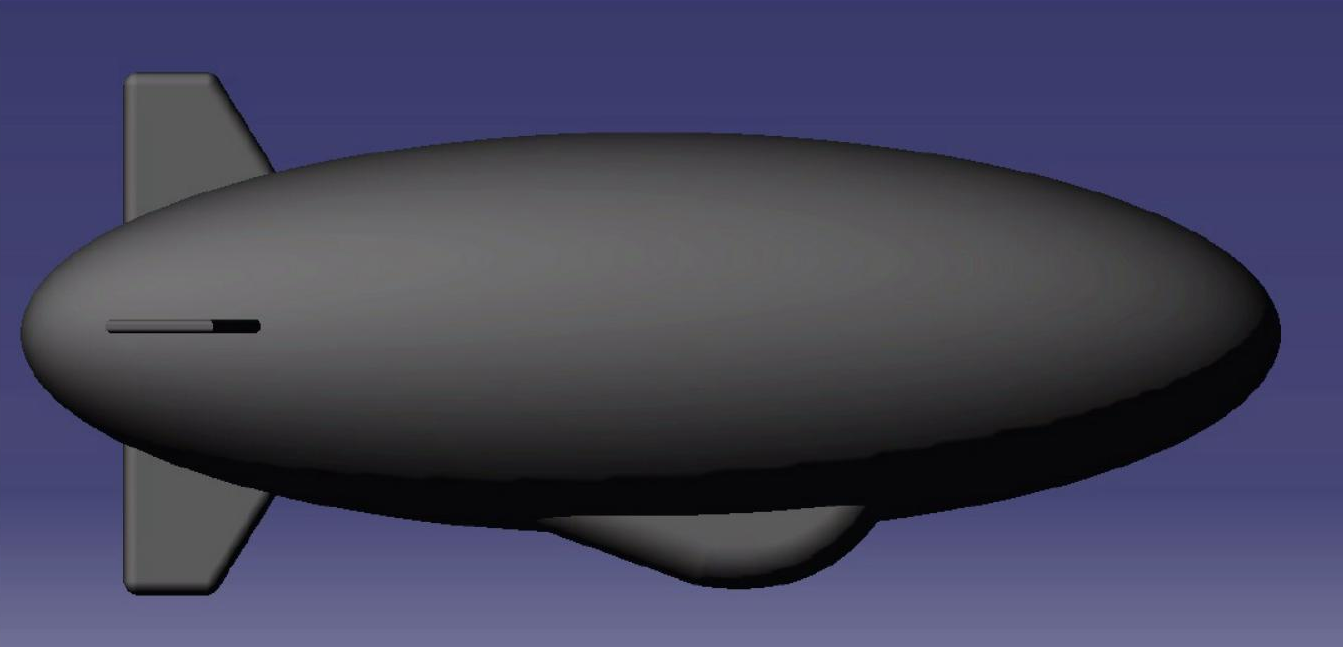
\includegraphics[scale=0.5]{figures/init.png}
\caption{Initial 3D sketch of the SPA concept}
\label{fig:init}
\end{figure}
%
\noindent
This simplified view of the mechanical design shows that it included the development of an envelope for the airship. The idea was to attach the solar panels on the top, mounted onto a wired mesh, with the cargo bay located at the bottom together with the propelling system.
\\
\\
However, due to new developments in the project that included the introduction of an already built blimp (envelope), the focus of the mechanical design was changed. The blimp to be used is the \textit{TIF-250} \cite{website:tif250}, shown in Figure \ref{fig:blimp}. This blimp has the capacity to lift a payload of about 2.5 kg, has a length of approximately 5 m and has a diameter (in the center) of about 1.9 m (see Table \ref{tab:technical}).
%
%\vspace{1.0em}
%
\begin{figure}[H]
\centering
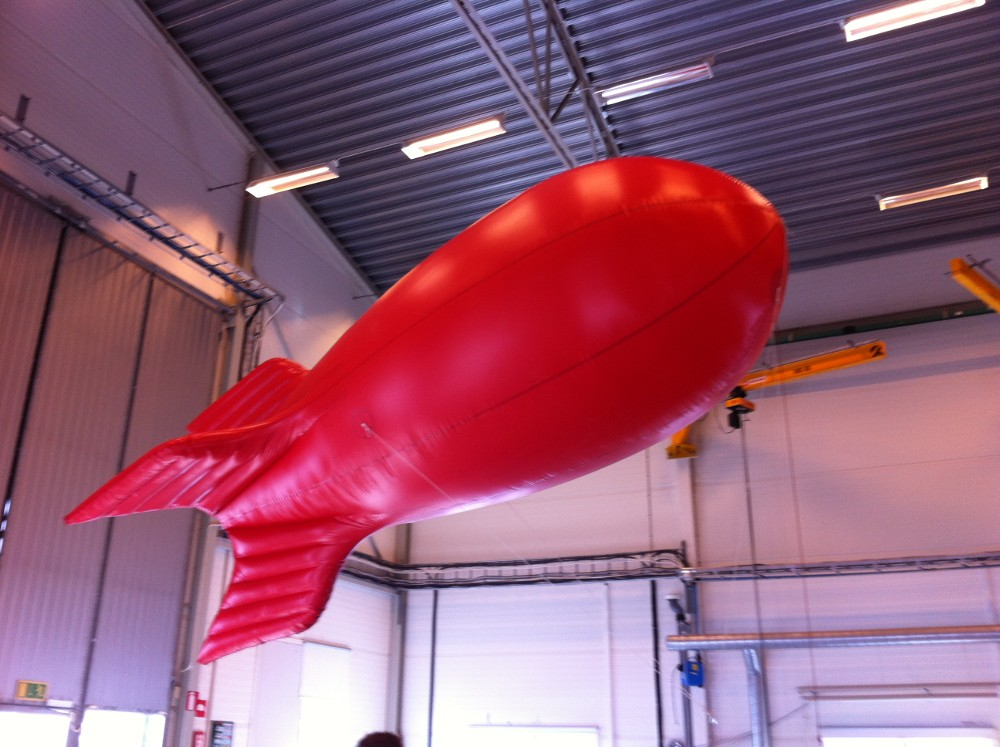
\includegraphics[width=0.8\textwidth]{figures/blimp.jpg}
\caption{Test of TIF-250 blimp from Esrange}
\label{fig:blimp}
\end{figure}
%
\noindent
This blimp serves the purpose of the U-SPACE project very well, as using it would allow to focus only on the construction of the support for the \ac{EPS}, on the cargo bay for the payload and on the integration of the propelling system. However, because it is a ready-built blimp with a purpose different than the one envisioned, it is not as lightweight as required. Nevertheless, light structures will be included in the integration of all other systems to remedy this problem.
%
\subsection{Envelope}
%
As was mentioned above, the blimp to be used is already built. This blimp is normally used to accurately measure the wind direction. Nevertheless it will have to fit the purpose of the U-SPACE project, due to the lack of time to build a new envelope. The blimp itself thus functions as the envelope.  
%
\subsection{Cargo Bay}
%
The cargo bay accommodates both the payload and the electronics required for \ac{U-SPACE}. The main challenge in the construction of this cargo bay is the mass. It has to be lightweight (the maximum total mass of all structures should be less than $1\,kg$) but at the same time rigid enough to resist some stress during the normal operation of the airship. To achieve this functionality, balsa wood reinforced with carbon fibres is used. Thermal cover film will be wrapped around the cargo bay. The current construction status is shown in Figure \ref{fig:cargo_bay}. 
%
\begin{figure}[H]
\centering
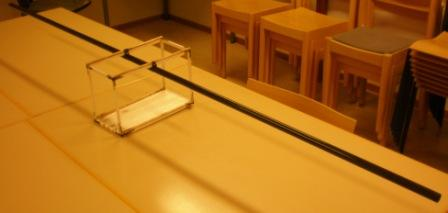
\includegraphics[width=\textwidth]{figures/fig_CDR_MSE_cargo_bay.jpg}
\caption{Current construction of the cargo bay} 
\label{fig:cargo_bay}
\end{figure}
%
%
\subsection{Power System}
%
The biggest challenge in this project is the accommodation of the power system, taking into account the maximum lift mass and the power requirements that consequently influence the solar panel quantity and mass. The idea is to use a lightweight wired mesh that serves as a support for the solar panels, which are attached to the wires with carbon fibre. This mesh is connected to the blimp by making use of three bands that will go around the blimp, distributing the weight along the envelope. These bands are made of fibre glass reinforced rubber tape. An idea of how the final design could look like is presented in Figure \ref{fig:mesh}.
%
%\pagebreak
%
\begin{figure}[bht]
\centering
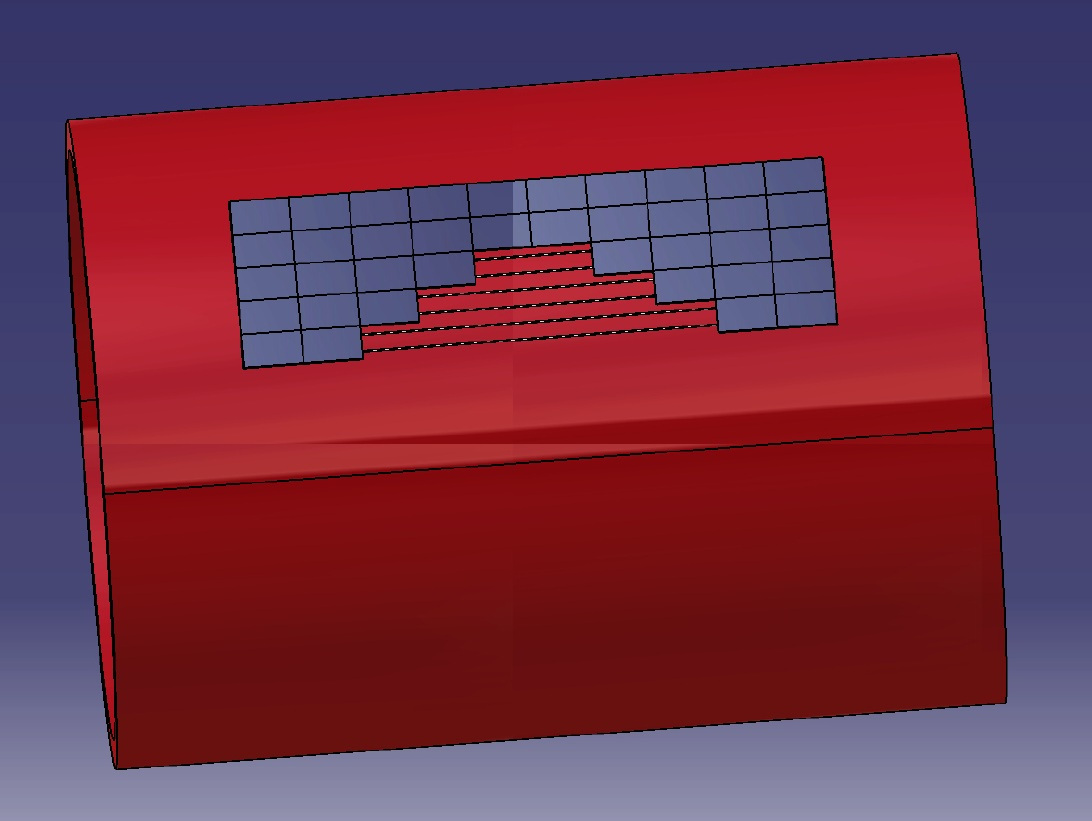
\includegraphics[scale=0.4]{figures/mesh.jpg}
\caption{3D sketch of the integration of the power system}
\label{fig:mesh}
\end{figure}
%
\subsection{Propelling System}
%
The propelling system is attached to a carbon fibre rod mounted onto the top of the cargo bay. The two motors are attached at the ends of the rod, away from the influence of the envelope and free to achieve their maximum aerodynamic capabilities. A hand sketch of this principle is shown in Figure \ref{fig:prop}.
%
\begin{figure}[h!]
\centering
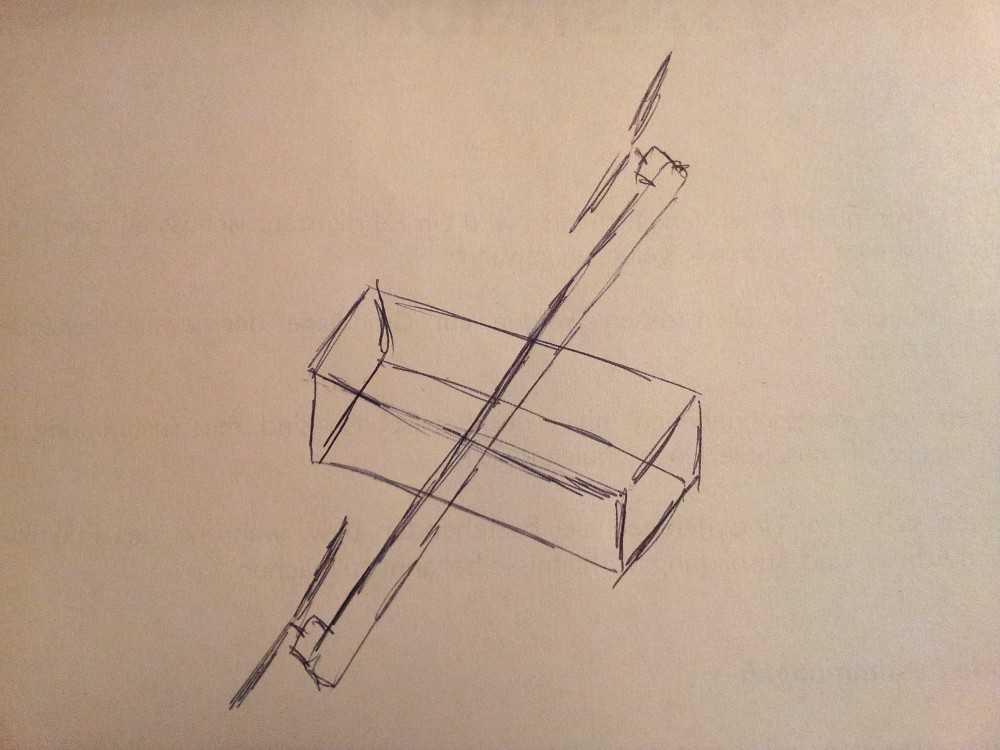
\includegraphics[scale = 0.3]{figures/prop.jpg}
\caption{Hand sketch of the integration of the propelling system}
\label{fig:prop}
\end{figure}
%
\subsection{Mass Budget}
%
A detailed mass budget of the U-SPACE subsystems and their components are listed in Table \ref{tab:mass_budget}.
%
\begin{table}[H]
\caption{U-SPACE mass budget}
\label{tab:mass_budget}
\begin{minipage}{\textwidth}
\centering
\begin{tabular}{llrr}
\hline
\textbf{Subsystem} & \textbf{Part} & \textbf{Weight} & \textbf{Budget}\\ 
\hline
EPS & Solar cells & $590-760\,g$\footnote{Depends on if solar cell with our without PSA is used} & \\
- & Battery & $122\,g$ & \\
- & Regulators + PCB & $55\,g$ & \\
- & Wiring & ? & \\
- & Mounting & $\sim 15\,g$ & \\
total: & & $952\,g$ & $1000\,g$\\
\hline
MCC & Motors + Propellers & $68\,g$ & \\
- & ESCs + Receivers & $21\,g$ & \\
- & Wiring & $5\,g$ & \\
- & Xbee-Pro radio  & $9\,g$ & \\
- & Motor attachments & $\sim 20\,g$ &  \\
total: & & $123\,g$ & $250\,g$\\
\hline
ITPU & BeagleBoard & $43\,g$ & \\
- & Sensors & $4\,g$ &  \\
- & PCB + Wiring & $30\,g$ &  \\
- & Etag & $39\,g$ &  \\
- & PCB Mounting & $\sim 20\,g$ & \\
total: & & $136\,g$ & $250\,g$ \\
\hline
MSE & Cargo Bay & $60\,g$ &  \\
- & Carbon rod & $191\,g$ &  \\
- & Envelope mesh & ? & - \\
- & Thermal insulation & $\sim 100\,g$ \\
total: & & $351\,g$ & $1000\,g$ \\
\hline\hline
system total: & & $1.551\,g$ & $2,500\,g$\\
\hline
\end{tabular}\par
\vspace{-0.75\skip\footins}
\renewcommand{\footnoterule}{}
\end{minipage}
\end{table}
%
\section{Future Developments}
%
%All the designs explained above have to be built and tested. 
%Design decisions have to be made and input from the other subsystems has to be taken into consideration. 
Only after a careful construction of the different structures that accommodate the required subsystems will it be possible to check if the requirement of the maximum lift mass (the most important requirement of this subsystem) is achieved. The 3D designs, the envisioned materials and previous experience in the field give hope that this constraint will be dealt with. 
The next steps are to finish the construction of the cargo bay, accommodate the propelling system and then to proceed with the construction of the wiring mesh and the attachment of the solar panels.
%
\section{Mechanical Interfaces}
%
The \ac{MSE} external mechanical interfaces and their planned implementations are listed in Table \ref{tab:mse_external_interfaces}.
%
\begin{table}[H]
\centering
\caption{\acl{MSE} external interfaces}
\label{tab:mse_external_interfaces}
\begin{tabular}{p{0.35\textwidth}p{0.6\textwidth}}
\hline
\textbf{External interface} & \textbf{Implementation}\\
\hline
Motors to carbon fiber rod & Attached on small aluminium plates that are fastened to carbon fiber rod using plastic clamps.\\
\rr Solar cells to envelope mesh & ? \tn
\rr Cargo bay to envelope mesh & ?\tn
Envelope mesh to blimp & ? \\
ITPU and EPS regulators to cargo bay & Attached with plastic spacers\footnote{For example \textit{1733427} from \url{www.farnell.com}} which are glued to cargo bay bottom plate.\\
Etag to cargo bay & Attached using the battery-housing to battery-sized piece which is glued to cargo bay bottom plate.\\
Battery and MCC receiver to cargo bay & Attached with Velcro glued to cargo bay bottom plate.\\
\hline
\end{tabular}
\end{table}
%
%\subsection{Mechanical Interface Control Drawing}
%
%Could not really find what this is and if we need it... Morten?
%
\subsection{Accommodation Requirements}
%
One of the main criteria for all mechanical assemblies is to minimize their weight. Thus low-weight materials like plastic, aluminium and carbon fiber are preferred. Secondly, all assemblies should be easy detachable for part replacement, changes in in mechanical layout, dissembling of subsystems for testing etc.
%
%\section{Physical Properties}
%
%E.g. mass in launch configuration...
%
%\section{Structural and Mechanisms Analysis}
%
%This involves things like dynamic analysis and stress analysis, but as we didn't really do this, just briefly comment on it...
%
%\section{Mounting Attachments}
%
%Not sure what they mean with this... Attachment concept and foot pattern?
\chapter{Electrical Power System}
\label{chap:eps}
%
\section{Introduction}
\label{sec:introduction}
%
The \ac{EPS} provides power to the motors, the on-board computer, the communication system and the payloads. Power is mainly supplied from solar cells but can also be supplied from a battery, when solar power is not available or insufficient. 
%
%\enlargethispage{2.0em}
%
\subsection{Changes from PDR to CDR}
\label{sec:changes_pdr_to_cdr}
%
Table \ref{tab:pdr_to_cdr} lists major design changes from the \ac{EPS} \ac{PDR} report.
%
\begin{table}[H]
\centering
\caption{Design changes from PDR to CDR}
\label{tab:pdr_to_cdr}
\begin{tabular}{p{0.2\textwidth}p{0.2\textwidth}p{0.5\textwidth}}
\hline
\textbf{Area of change} & \textbf{Change} & \textbf{Argumentation for change}\\
\hline
\rr Total power budget & \rr Increased to $>40\,W$ & Airship total mass and size are increased thus requiring much more power for the motors.\tn
Solar cells & New part & \rr Old solar cell was much heavier than listed in manufacturer datasheet due to a glass cover.\tn
Total system cost & \rr Increased to $>12000\,SEK$ & \rr Increased power and new light-weight solar cells are more expensive.\tn
\rr Solar cell mounting & New part & \rr New solar cell is flexible instead of rigid and can be mounted with \ac{PSA}.\tn
Battery & New part & \rr A battery that supports much higher discharge currents has been selected which simplifies current limiting circuitry and improves battery efficiency.\tn
\hline
\end{tabular}
\end{table} 
%
%
\section{Functional and Technical Requirements}
\label{sec:requirements}
This section describes the functional and technical \ac{EPS} requirements along with the expected \ac{EPS} performance.
%
\subsection{Functional Requirements}
The primary functional \ac{EPS} requirements are:
%
\begin{itemize}
\item Provide adequate power to motors, other subsystems and payloads
\item Prove that flying on solar energy is possible i.e more power produced than consumed
\end{itemize}
%
Additional desired requirements are:
%
\begin{itemize}
\item Scalable and flexible system architecture allowing the \ac{EPS} to be upgraded to higher power levels or re-used in different applications (rover, \ac{UAV} etc.)
\item Robust design allowing flight in more extreme conditions (altitude, weather etc.)
\item Provide adequate protection circuits for battery and loads to prevent any major failure and damage to other subsystem components.
\item Optimal design and high performance to increase power capability and minimize system mass
\end{itemize}
%
\subsection{Power Budget and Technical Requirements}
%
The \ac{EPS} power budget is listed in Table \ref{tab:power_budget} and the technical requirements are listed in Table \ref{tab:technical_requirements}.
%
%
\begin{table}[H]
\centering
\caption{Power budget}
\label{tab:power_budget}
\begin{tabular}{lrr}
\hline
\textbf{Part/subsystem} & \textbf{Peak load} & \textbf{Average load}\\
\hline
2 x \ac{MCC} motors & $120\,W$ & $\sim 40\,W$ \\
\ac{MCC} ETag & $100\,mW$ & $100\,mW$ \\
\ac{MCC} Xbee-Pro radio & $10\,mW$ & $10\,mW$ \\
\rr \ac{ITPU} BeagleBoard + sensors & $3\,W$? & $3\,W$?\tn
\hline\hline
Total: & $123.11\,W$ & $43.11\,W$ \\
\hline
\end{tabular}
\end{table}
%
%
\begin{table}[H]
\centering
\caption{Technical requirements for EPS}
\label{tab:technical_requirements}
\begin{minipage}{\textwidth}
\begin{tabular}{p{0.3\textwidth}p{0.15\textwidth}p{0.45\textwidth}}
\hline
\textbf{Description} & \textbf{Symbol} & \textbf{Value}\\
\hline
Minimum power output & $P_{out,min}$ & $40\,W$\footnote{Average \ac{SAR} output power including losses}\\
Maximum mass & $W_{EPS,max}$ & $1000\,g$ including solar array\\
Maximum cost & - & $4000\,SEK$\footnote{Initial budget for 2 students}\\
Output voltages & $V_{mainbus}$, $V_{5V}$ & $6.0-9.5\,V$ un-regulated and $5\,V$ regulated\\
Operational temperature & $T_{min}$, $T_{max}$ & $-20^{\circ}C\;to\;+45^{\circ}C$\\
Battery capacity & $C_{bat}$ & $>5\,Wh$\\
\hline
\end{tabular}\par
\vspace{-0.75\skip\footins}
\renewcommand{\footnoterule}{}
\end{minipage}
\end{table}
%
%
%
\subsection{Mission and Environmental Constraints}
\label{subsec:environmental_requirements}
This section discusses the system challenges imposed by the operation environment.
%
\subsubsection*{Solar Array Temperature}
As was discussed in \cite{PDR}, the optimal operating voltage of the solar cells change with temperature. The \ac{EPS} must be able to generate optimal power from the solar cells in the full expected temperature range of the environment. This can be achieved using a \ac{MPPTU} which will be discussed in section \ref{sec:MPPTU}
%
\subsubsection*{Solar Incidence Angle}
The flight location of U-SPACE is near Kiruna in Sweden. Figure \ref{fig:SolarIncidenceAngles} shows the average solar incidence angles in Kiruna for the months June and September \cite{web:solarincidence}, considering a flat solar panel facing straight up.
The solar cell output current drops with the Kelly cosine function as shown in Figure \ref{fig:KellyCosine}. To minimize power losses due to inclined solar incidence, the \ac{MSE} design must consider the optimal mounting position and angle of the solar panels. The most optimal flight conditions are at noon in June, with a solar incidence angle of around $46^{\circ}$. However, this still reduces the solar array output by about $30\%$. If the solar array output should not drop by more than $50\%$, the maximum solar incidence angle is about $57^{\circ}$. This is only an approximation from the assumption that the solar array is mounted flat on top of the airship envelope, which will not be the exact case in practice.
%
\begin{figure}[H]
\centering
\begin{minipage}[t]{0.48\linewidth}
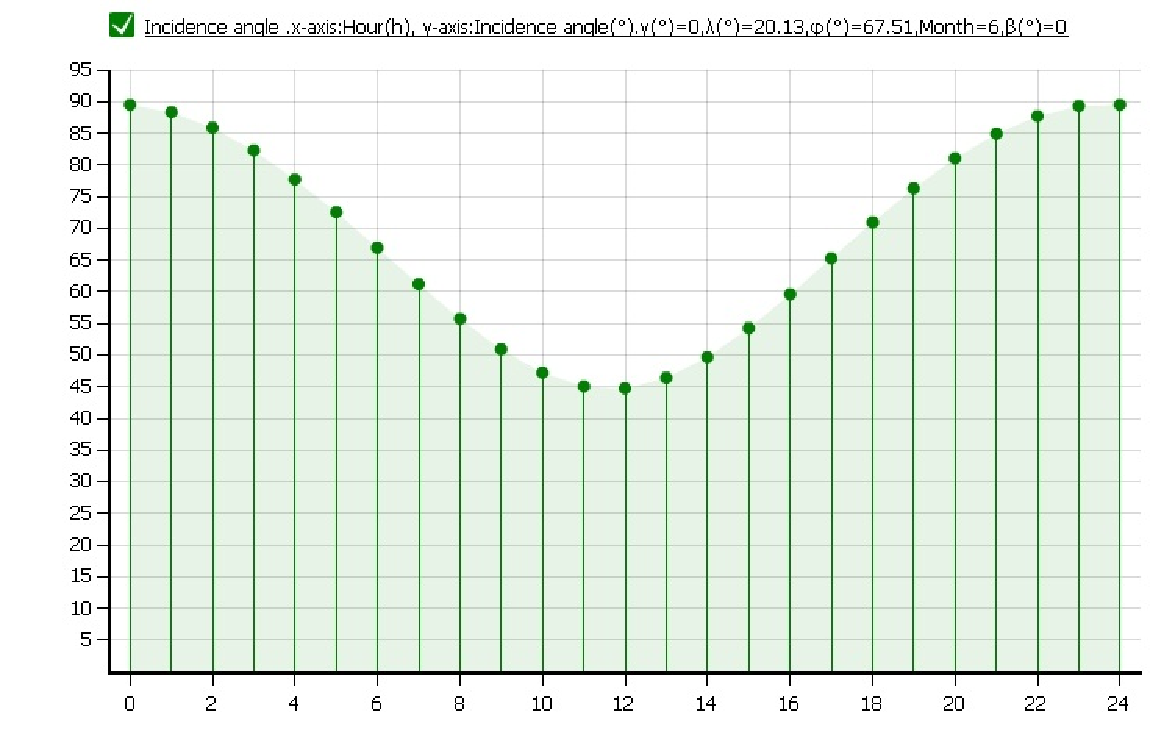
\includegraphics[width=\textwidth]{figures/fig_CDR_EPS_SolarIncidenceAngle_Jun}
\end{minipage}
%\vspace{0.5mm}
\begin{minipage}[t]{0.48\linewidth}
\centering
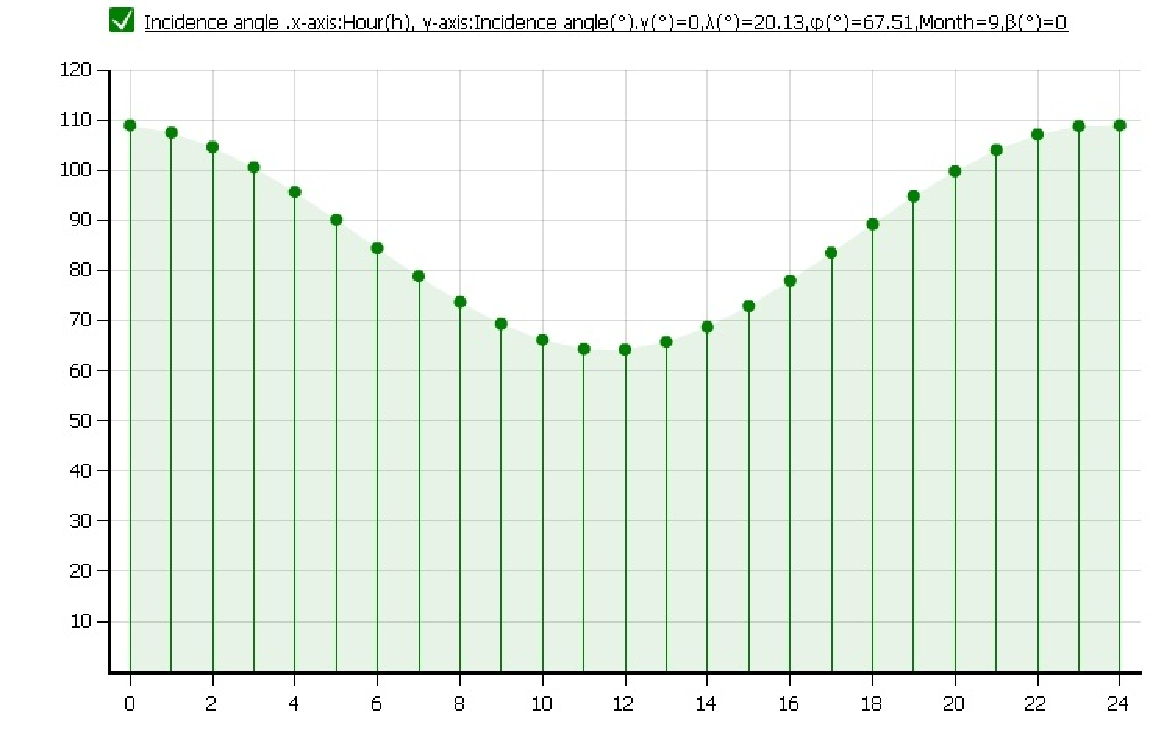
\includegraphics[width=\textwidth]{figures/fig_CDR_EPS_SolarIncidenceAngle_Sep}
\end{minipage}
\caption[Solar incidence angles]{Monthly average solar incidence angles for June (left) and September (right) for each hour of the day.}
\label{fig:SolarIncidenceAngles}
\end{figure}
%
\begin{figure}[H]
\centering
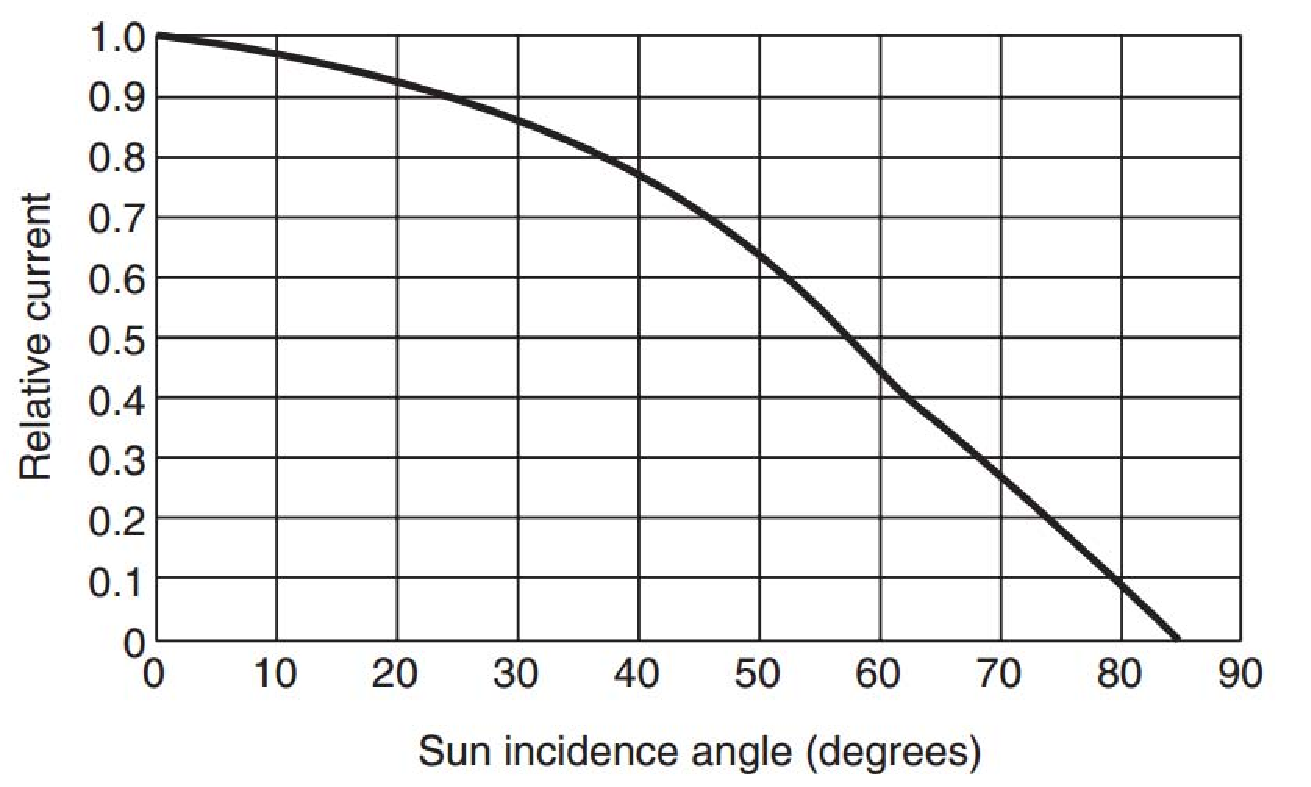
\includegraphics[scale=0.4]{figures/fig_KellyCosine}
\caption[Kelly cosine function]{Kelly cosine function showing how solar cell photo current depends on sun incidence angle onto the solar cell\cite[Fig 9.12]{book:mukund_wind}}
\label{fig:KellyCosine}
\end{figure}
%
%
\subsubsection*{Solar Array Shading}
Shading on the solar panels, for example caused by airship stabilizer structures or objects in the landscape, can cause a significant drop in the cell output voltage, as described in \cite[p. 165]{Mukund}. Bypass diodes can be used to partly mitigate this issue. However, since the airship is only expected to fly at altitudes above normal terrain and building height the only shading possibly expected is from the airship structure. Hence the \ac{MSE} design must consider this restriction.
%
\subsubsection*{Battery Temperature}
One of the most temperature-critical \ac{EPS} components is the battery, which must stay within its safety temperature limits. In the proposed design, only temperature monitoring is offered. Therefore, flight is only allowed when outdoor temperatures are well within the allowed battery temperature range. Otherwise a battery heater and more sophisticated thermal design may be necessary.
%
\subsection{Expected Performance}
The expected \ac{EPS} performance values are listed in Table \ref{tab:expected_performance}.
%
\begin{table}[H]
\centering
\caption{Expected performance for the \ac{EPS}}
\label{tab:expected_performance}
\begin{minipage}{\textwidth}
\begin{tabular}{p{0.4\textwidth}p{0.15\textwidth}p{0.35\textwidth}}
\hline
\textbf{Description} & \textbf{Symbol} & \textbf{Value}\\
\hline
Power conversion efficiency (SAR) & - & $>90\%$\\
Power output (SAR) & $P_{out}$ & $\sim 45\,W$\footnote{For ideal weather conditions, i.e. no clouds and best expected solar incidence angle}\\
Battery capacity & $C_{bat}$ & $7.3\,Wh$\\
Mass & $W_{EPS}$ & $\sim980\,g$\\
Total cost & - & $\sim12000\,SEK$\footnote{Solar cells are significantly more expensive than anticipated. A request for more funds is under preparation.}\\
\hline
\end{tabular}\par
\vspace{-0.75\skip\footins}
\renewcommand{\footnoterule}{}
\end{minipage}
\end{table}
%
%
\section{Critical Design}
\label{sec:critical_design}
%
The basic \ac{EPS} diagram is shown in  Figure \ref{fig:EPS_diagram_simple}. A \ac{SAR} controls the operating voltage of the solar array and supplies an un-regulated mainbus. The mainbus voltage is mainly controlled by the battery voltage. A DC-DC regulator provides a regulated $5\,V$ supply to subsystems and payloads. The motors are supplied from the unregulated mainbus.
%
\begin{figure}[H]
\centering
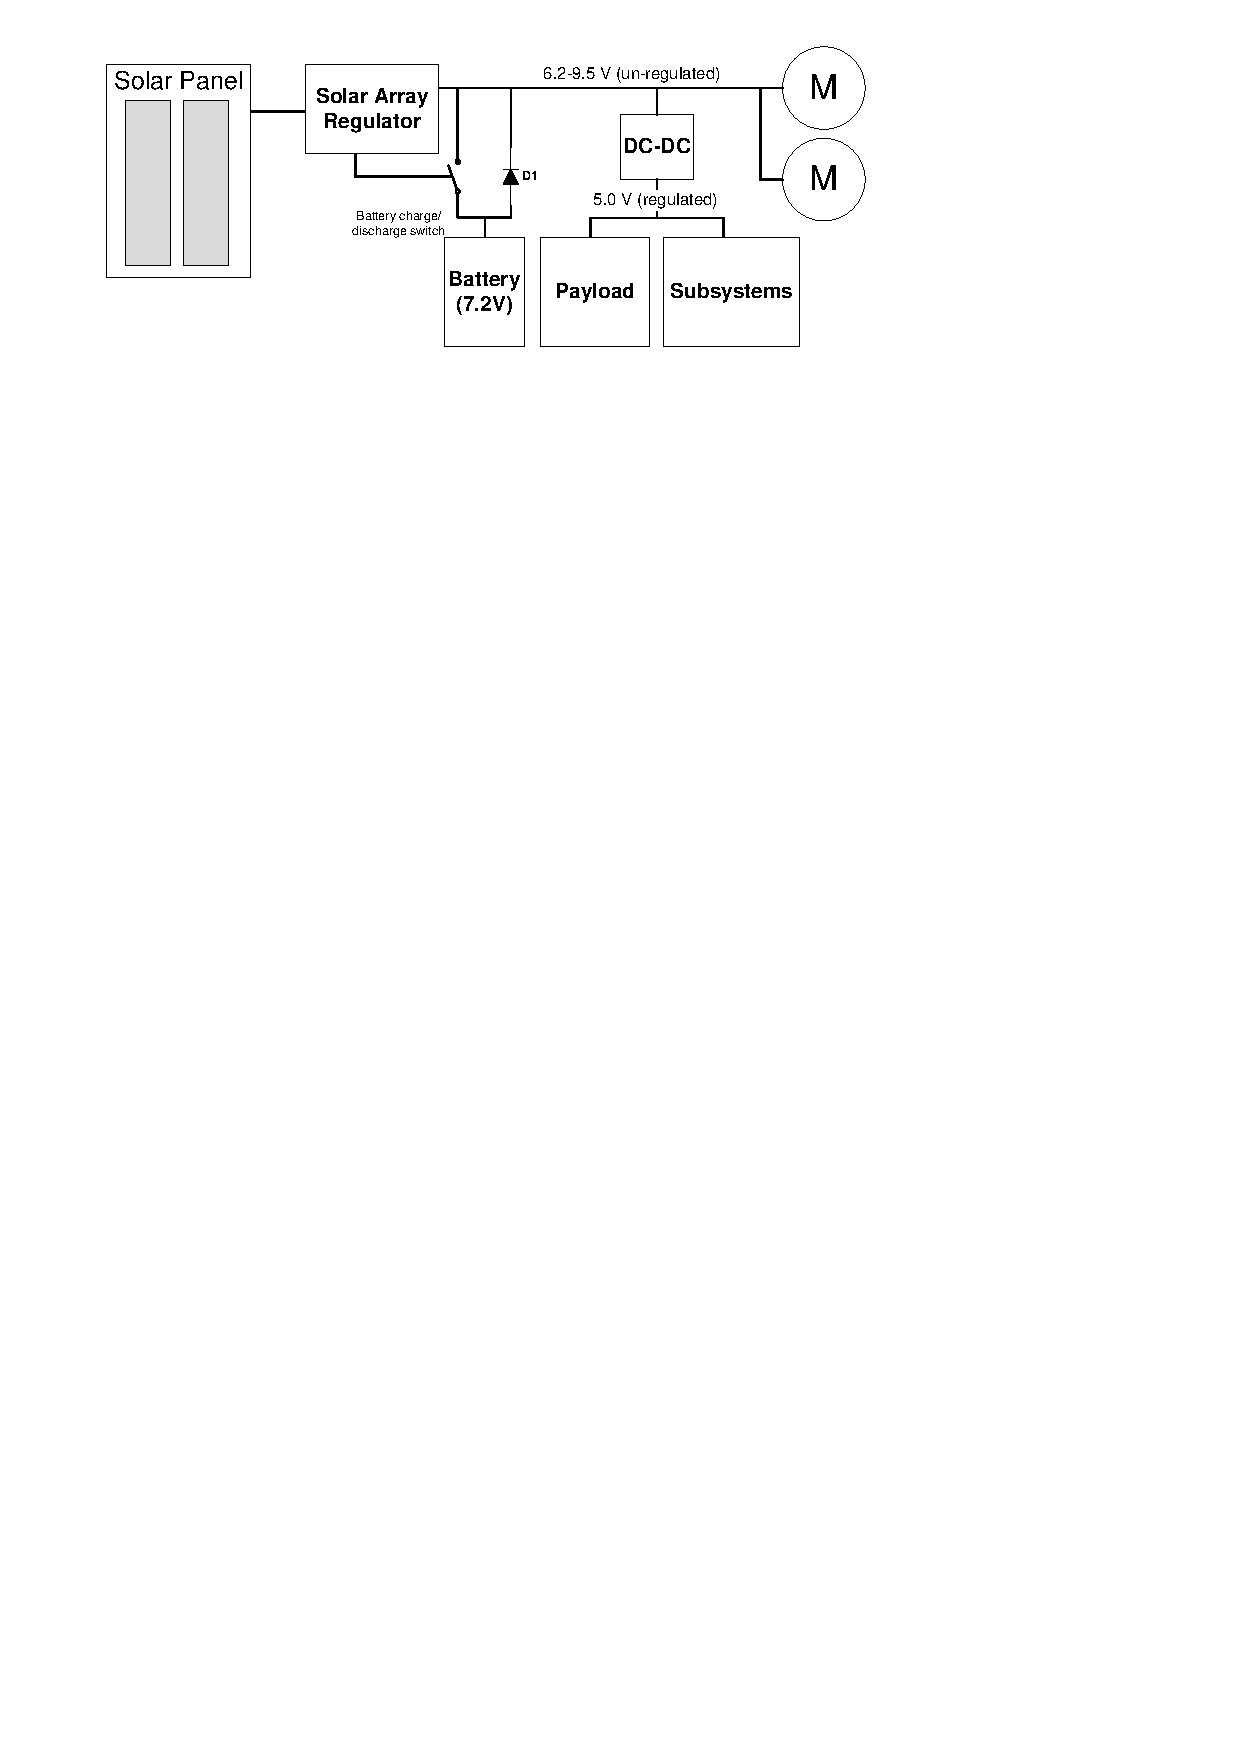
\includegraphics[width=\textwidth]{figures/fig_PDR_EPSdiagram}
\caption{EPS simple block diagram}
\label{fig:EPS_diagram_simple}
\end{figure}
%
%
\subsection{Battery Design}
In \cite{PDR} it was decided that a Li-ion type battery was suitable for the \ac{EPS}. An \textit{Ansmann \ac{LiPo} Racing Pack 2S1P 30C} battery is selected with the specifications as listed in Table \ref{tab:proposed_battery}.
%
\begin{table}[H]
\centering
\caption{Specifications of selected battery}
\label{tab:proposed_battery}
\begin{tabular}{p{0.35\textwidth}p{0.15\textwidth}p{0.4\textwidth}}
\hline
\textbf{Description} & \textbf{Symbol} & \textbf{Value}\\
\hline 
Chemistry & - & Li-Polymer\\
Nominal voltage & $V_{bat}$ & $7.4\,V$\\
Capacity & $C_{bat}$ & $2.1\,Ah$ / $15.54\,Wh$\\
Weight & $W_{bat}$ & $122\,g$\\
Dimensions & - & $105\,mm\:\times\:35.2\,mm\:\times\:17\,mm$\\
Maximum fast charge current & $I_{charge,max}$ & $3\,A$\\
\rr Maximum discharge current (continuous) & $I_{discharge,max}$ & $63\,A$\\
\hline
\end{tabular}
\end{table}
%
%
\subsubsection{Battery Charge Regulator}
\label{subsec:BCR}
%
The \ac{BCR} must control the charge rate of the battery such that the charge current limit is not exceeded and it must cut off the charge current when the battery is fully charged. Temperature monitoring is usually also required to inhibit charging if the battery temperature is outside its safety limits. 
\\
\\
A \textit{MCP73842} Li-ion battery charge regulator \ac{IC} is selected. It employs three different charge modes: low-charge for deeply discharged batteries, \ac{CC} charge and trickle charging. It also includes inputs for temperature monitoring. The battery maximum charge current was given in Table \ref{tab:proposed_battery} as $3\,A$. From the \textit{MCP73842} datasheet, the minimum current sense resistor, $R_{sense}$, is calculated as
%
\begin{equation}
R_{sense}=\dfrac{V_{FCS}}{I_{REG}}=\dfrac{120\,mV}{3\,A}=40\,m\Omega
\end{equation}
%
Where $V_{FCS}$ is the fast charge voltage regulation across the sense resistor and $I_{REG}$ is the desired charge current. A $50\,m \Omega$ current sense resistor is selected leading to a charge current of $2.4\,A$. A heat sink must be added according to the thermal calculations in Appendix \ref{app:BCR_trans_max_heat_dissipation}.
%
In Appendix \ref{app:BCR_trans_max_heat_dissipation}, heat sink requirements for the \ac{BCR} transistor are calculated.
%
\subsubsection*{Future Improvements}
As was calculated above, significant power may be lost in the \ac{BCR} \ac{MOSFET}. This is due to the selected \ac{BCR} \ac{IC} which requires an input voltage of around $9.5\,V$ (including a Schottky diode forward voltage drop and some design margin). In the future, the \ac{BCR} could be designed to allow operation with an input voltage only slightly above the battery voltage thus minimizing the charge losses and relaxing the thermal requirements of the \ac{MOSFET}.
%
%
\subsubsection{Battery Temperature Monitoring}
%%
The selected \ac{LiPo} battery is rated, in charge-mode, for the temperature interval $0$ to $+45^{\circ}C$. For temperature measuring, a $4.7\,k \Omega$ \textit{NTCLE203E3472GB0} thermistor is selected which has a Beta Value, $B=3977\,K$. Since the battery temperature is measured using an external thermistor, the temperature response is likely to be somewhat slower, so an extra $5^{\circ}C$ thermal design margin is added. The required resistance values of the \ac{BCR} temperature control resistors are determined from the \textit{MCP73842} datasheet as 
%
\begin{equation}
\begin{split}
R_{cold}&=R_{25}\,e^{B(\dfrac{1}{T}-\dfrac{1}{T_0})}=4.7\,k\Omega \,e^{3977\,K(\dfrac{1}{278	\,K}-\dfrac{1}{298\,K})}=12.28\,k\Omega\\
R_{hot}&=4.7\,k\Omega \, e^{3977\,K(\dfrac{1}{313	\,K}-\dfrac{1}{298\,K})}=2.48\,k\Omega\\
R_{T1}&=2\dfrac{R_{cold}R_{hot}}{R_{cold}-R_{hot}}=6.2\,k\Omega\\
R_{T2}&=2\dfrac{R_{cold}R_{hot}}{R_{cold}-3R_{hot}}=12.6\,k\Omega
\end{split}
\end{equation}
%
where $R_{25}$, $R_{cold}$ and $R_{hot}$ are the thermistor resistance values at room temperature, the low and high temperature limits respectively. $R_{T1}$ and $R_{T2}$ are the required \ac{BCR} temperature control resistors setting the required temperature interval.
\\
\\
If the sensed battery temperature falls outside the $+5$ to $+40^{\circ}\,C$ region, battery charging will be inhibited. The technical requirements from Table \ref{tab:technical_requirements} require the \ac{EPS} to operate down to $-20^{\circ}\,C$. Hence some insulation and/or heating of the battery may be necessary or flight must be disallowed at outdoor temperatures much below $+5^{\circ}\,C$.
%
\subsubsection{Battery Under-Voltage Lock-Out}
To prevent over-discharge of the battery, a battery \ac{UVLO} circuit is added as shown in Figure \ref{fig:EPS_diagram_detailed}. An \textit{TL431} precision shunt regulator \ac{IC} is selected. The lock-out voltage is given as
%
\begin{equation}
V_{UVLO}=V_{ref}(1+\dfrac{R_1}{R_2})=2.5\,V(1+\dfrac{29\,k \Omega}{20\,k \Omega})=6.125\,V
\end{equation}
%
where $V_{ref}$ is the \textit{TL431} built-in voltage reference. If the battery voltage drops below this value, the gate voltage to the P-type \ac{MOSFET} is pulled high, thus opening the switch. The $1\,M \Omega$ resistor adds about $200\,mV$ hysteresis. 
\\
\\
The \ac{UVLO} circuit only cuts out the motor power line. Thus payloads remain supplied and the battery is still slowly drained. This design has been chosen to allow  telemetry and telecommand capability during a heavy battery discharge event. In this case, it is expected that all payloads and on-board computers enter a low power consumption mode, to extend the remaining battery supply time. If the battery voltage drops below $5.62\,V$, the $5\,V$ payload power supply shuts down and all telemetry and telecommand capabilities will be lost.
%
%\pagebreak
%
\subsection{Solar Array Design}
\label{sec:SA}
The main driver for selecting the solar cell is to choose a part which is very lightweight and easy to mount on the \ac{SPA}. A  \textit{PowerFilm RC7.2-75 (PSA)} solar cell is selected as shown in Figure \ref{fig:solar_cell}. This is a very lightweight flexible solar cell with a \ac{PSA} backside for mounting. Table \ref{tab:solar_cell_spec} lists the solar cell specifications.
%
\begin{table}[H]
\centering
\caption{Specifications of selected solar cell}
\label{tab:solar_cell_spec}
\begin{minipage}{\textwidth}
\begin{tabular}{p{0.35\textwidth}p{0.15\textwidth}p{0.4\textwidth}}
\hline
\textbf{Description} & \textbf{Symbol} & \textbf{Value}\\
\hline
Nominal output current & $I_{cell}$ & $100\,mA$\\
Nominal output voltage & $V_{cell}$ & $7.2\,V$\\
Nominal output power & $P_{cell}$ & $0.72\,W$\\
Dimensions & - & $270\,mm\:\times\:90\,mm\:\times\:0.2\,mm$\\
Weight & $W_{cell}$ & $7.6\,g$\\
No. of required cells & $N_{cells}$ & $100$\footnote{\cite{avnetexpress} offers good discount for +100 units order}\\
Total solar array area & $A_{array}$ & $2.43\,m^2$ (assuming $100\,\%$ fill factor)\\
\hline
\end{tabular}\par
\vspace{-0.75\skip\footins}
\renewcommand{\footnoterule}{}
\end{minipage}
\end{table}
%
\noindent
The solar array is an array of 50 parallel connected strings of two series solar cells as shown in Figure \ref{fig:solar_cell}. The nominal output voltage and current are given as
%
\begin{equation}
\begin{split}
V_{array}&=2\cdot V_{cell}=14.4\,V\\
I_{array}&=50\cdot I_{cell}=5\,A
\end{split}
\end{equation}
%
\begin{figure}[H]
\centering
\begin{minipage}[c]{0.4\linewidth}
\centering
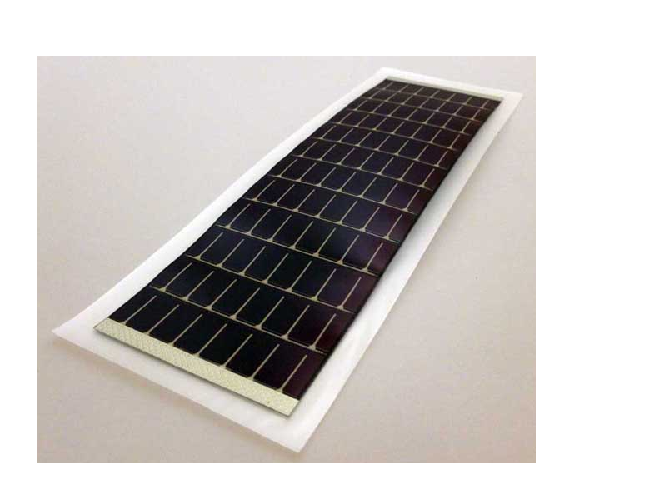
\includegraphics[width=\textwidth]{figures/SolarCell_RC7-2_Powerfilm}
\end{minipage}
\hspace{5mm}
\begin{minipage}[c]{0.55\linewidth}
\centering
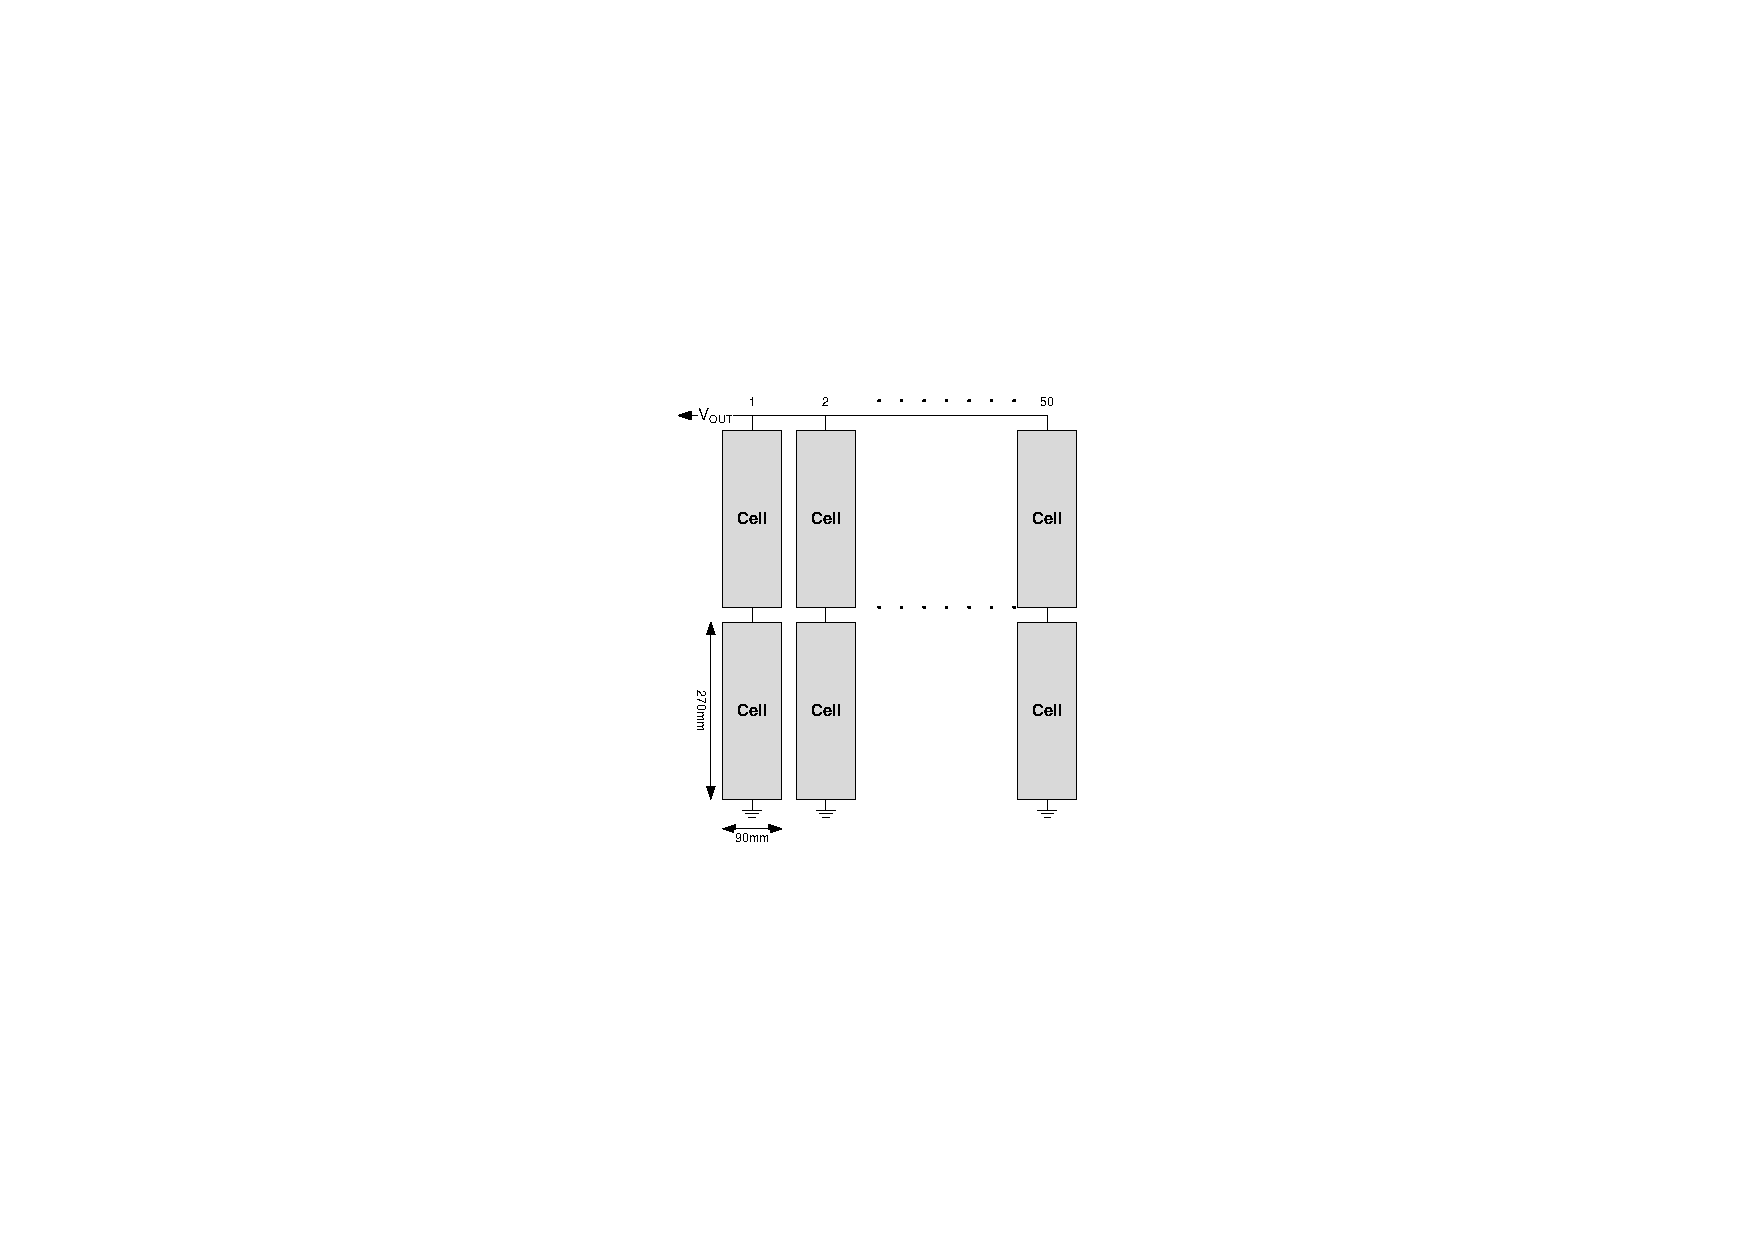
\includegraphics[width=0.9\textwidth]{figures/fig_CDR_Solar_Array}
\end{minipage}
\caption[PowerFilm solar cell and solar array configuration]{PowerFilm solar cell (left) and solar array configuration (right)}
\label{fig:solar_cell}
\end{figure}
%
\noindent
Bypass diodes were briefly discussed in section \ref{subsec:environmental_requirements}.
But since only two cells are connected in series, it is estimated that bypass diodes are not very important in mitigating shading issues since it would require a large amount of diodes (one for every solar cell string) and only one cell is bypassed.
%
\subsection{Solar Array Regulator}
The \ac{SAR} must control the optimal solar array operating voltage as well as limit the output mainbus voltage. A simple step-down buck converter topology is preferred for a number of reasons:
%
\begin{itemize}
\item simple circuit analysis and low components count
\item no inherent \ac{RHPZ} in contrary to the standard boost topology
\item step-down topology calls for a high input voltage which leads to low input current thus minimizing ohmic losses and the relative forward voltage drop loss from the reverse protection diode
\end{itemize}
%
\subsubsection{Buck Converter Circuit Design}
The ideal transfer function for the buck converter shown in Figure \ref{fig:EPS_diagram_detailed} is given as
%
\begin{equation}
V_{out}=D\,V_{in}
\end{equation}
%
where $D$ is the duty cycle of the \ac{MOSFET} switch, $V_{in}$ the solar array voltage and $V_{out}$ the mainbus voltage. The duty cycle is controlled by a \ac{PWM} controller which provides input to a high-side \ac{MOSFET} driver. A \ac{MEA} measures the mainbus output voltage to generate a control signal for the PWM controller. An \textit{LM3477} chip is selected which combines \ac{PWM} controller, \ac{MEA} and gate driver in one \ac{IC}.
\\
\\
The \ac{CM} control scheme is adopted due to its excellent dynamic abilities \cite[sec. 12-3-6]{Fundamentals} and simplified feedback regulator design. A $10\,m \Omega$ precision sense resistor measures the inductor current slope. The \textit{LM3477} has built-in slope compensation to avoid current mode instabilities \cite[sec. 12-1]{Fundamentals}.
\\
\\
The converter switching frequency, $f_{switch}$, is chosen relatively high to $500\,kHz$. The increased switching losses are expected to be outweighed by the fact that the low operating voltage limits switching losses and the high frequency allows the inductor and filter components to be made smaller, thus limiting system mass and the resistive losses in the inductor copper wires which are expected to dominate the converter losses due to the relatively high currents. The inductor current ripple, $\Delta I_L$, can be calculated as 
%
\begin{equation}
\Delta I_L=\dfrac{V_{in}-V_{out}}{L\,f_{switch}}D
\end{equation}
%
where $L$ is the inductance and $f_{switch}$ the converter switching frequency. 
The inductor current ripple is usually limited to about $10\,\%$ of the maximum converter output current leading to a minimum required inductance of
%
\begin{equation}
L=\dfrac{V_{in}-V_{out}}{\Delta I_L\,f_{switch}}D=\dfrac{14.4\,V-7.4\,V}{10\% \cdot 10.83\,A\cdot 500\,kHz}\cdot 0.514=6.7\,uH
\end{equation}
%
where $10.83\,A$ is the maximum converter output current calculated as 
%
\begin{equation}
I_{SAR,max}=\dfrac{P_{out,max}}{V_{out,min}}=\dfrac{65\,W}{6.0\,V}=10.83\,A
\end{equation}
%
A $10\,uH$ inductor is chosen giving a current ripple of about $0.72\,A$. If the load current drops below $0.36\,A$, which is unlikely to happen in most operating modes, the converter will enter \ac{DCM}.
\\
\\
For the converter output capacitor, a component is chosen which has very low \ac{ESR} and high capacitance to limit the output voltage ripples.
%
\subsubsection*{Current Sense Amplifier}
With an inductor current ripple of $0.72\,A$ the current sense voltage slope is only 
%
\begin{equation}
v_{sense}=\Delta I_L\cdot R_{sense}=0.72\,A\cdot 10\,m\Omega = 7.2\,mV
\end{equation}
%
It is recommended that the slope compensation is equal to or the double of the sense slope \cite[sec. 12-1]{Fundamentals}, however the minimum compensation slope is limited to $103\,mV$ by the \textit{LM3477} chip. Thus the sensed slope signal must be amplified, with a gain of around 20 being suitable. This also has the advantage of eliminating some of the typical noise susceptibility in the current sense signal. The current sense circuit in Figure \ref{fig:EPS_diagram_detailed} consists of two differential OpAmps which amplify the current sense slope. Resistive voltage dividers are placed on the OpAmp inputs to scale down the input voltage signals to always be below the $5\,V$ OpAmp supply voltage.
\\
\\
Since a closed-loop OpAmp gain of 20 is needed at an operating frequency of $500\,kHz$, the gain-bandwidth specification of the OpAmps must be more than $10\,MHz$. The \textit{LTC6362CMS8PBF} OpAmp is selected. One limitation of this OpAmp is its temperature range which only goes down to $0^{\circ}\,C$. This might be solved by thermally connecting it to the transistor heat sinks or by ensuring that the internal \ac{EPS} temperature does not go below $0^{\circ}\,C$.
%
\subsubsection*{Input Filter}
An input filter is placed in front of the buck converter, mainly to draw a continuous current from the solar array. It also reduces the converters \ac{EMC} issues (see chapter \ref{chap:emc}). One challenge with the input filter is that it affects the dynamic properties of the converter and if not properly designed, it can degrade the control feedback loop performance. A damping network in the filter is also necessary to avoid instabilities \cite[sec. 10-3]{Fundamentals}.
\\
\\
A usable filter has been designed based on PSpice simulations. However thorough analysis still remains to be done to optimize the filter design.
%
%
\subsubsection{Maximum Power Point Tracking Unit}
\label{sec:MPPTU}
In \cite{PDR} it was decided to use a \ac{MPPTU} with the \ac{SAR} to increase solar array efficiency during changing environmental conditions. The \ac{SAR} with \ac{MPPT} can operate in three different operation regions:
%
\begin{itemize}
\item Battery discharge - when the solar array input power is insufficient to cover the load power demand, the battery is slowly discharged in order to maintain the output voltage. The \ac{MPPTU} controls the input solar array voltage.
\item Battery charge - when the solar array input is greater than the load power, excessive power is used to recharge the battery. The \ac{MPPTU} controls the input solar array voltage.
\item Input power limitation - when the battery is fully charged, the regulator will operate the solar array at a non-optimal voltage, thus limiting the input power to keep the output voltage at a maximum limit. The extra potential input power is dissipated as heat externally on the solar arrays.
\end{itemize}
%
It is preferred to implement an analog \ac{MPPTU} mainly since this makes the circuit independent of a control signal from a more complicated external \ac{MCU} or \ac{DSP}, thus allowing a flexible plug'n-play system to be implemented. One challenge with an analog \ac{MPPTU} is the typical need for expensive analog multipliers \cite{Liang}. Since the required multiplier only needs to be a first quadrant type (only two positive inputs), it is believed that a low-cost multiplier can be built using standard discrete components \cite{Multiplier}.
%
\\
\\
The \ac{MPPTU} design still remains to be completed.
%
%
\subsubsection{Mode Transitions}
%
As was discussed in Section \ref{sec:MPPTU}, the \ac{SAR} can operate in three different main modes. The transition between the modes is controlled by the mainbus output voltage as shown in Figure \ref{fig:SAR_ModeTransition}. If the \ac{SAR} input power is lower than the load power, the battery will discharge and the mainbus voltage will follow the battery voltage. Once the input power is larger than the load power, the mainbus capacitor will quickly be charged to a voltage higher than the battery voltage. Once the mainbus capacitor voltage crosses the $9.2\,V$ charge threshold, the \ac{BCR} starts to charge the battery. If the input power is still higher than the combined battery charge power and load power, the mainbus capacitor voltage continues to rise until reaching $9.5\,V$ where the \ac{SAR} enters the input power limitation mode. The battery may still be charging in this mode. Since the battery is charged with constant current, the input power may be lower than the combined charge and load power but higher than the load power alone. Hence an oscillatory state between battery charge and discharge mode may arise, whose frequency depends on the mainbus capacitance which should therefore be large. 
\\
\\
The $9.20\,V$ battery charge threshold voltage is calculated from
%
\begin{equation}
V_{charge,threshold}=V_{UVLO,BCR}+V_F=8.90\,V+0.3\,V= 9.20\,V
\end{equation}
%
where $V_{UVLO,BCR}$ is the worst-case \ac{UVLO} threshold voltage of the \ac{BCR} \ac{IC} and $V_F$ is the reverse protection diode forward voltage drop.
%
%
\begin{figure}[H]
\centering
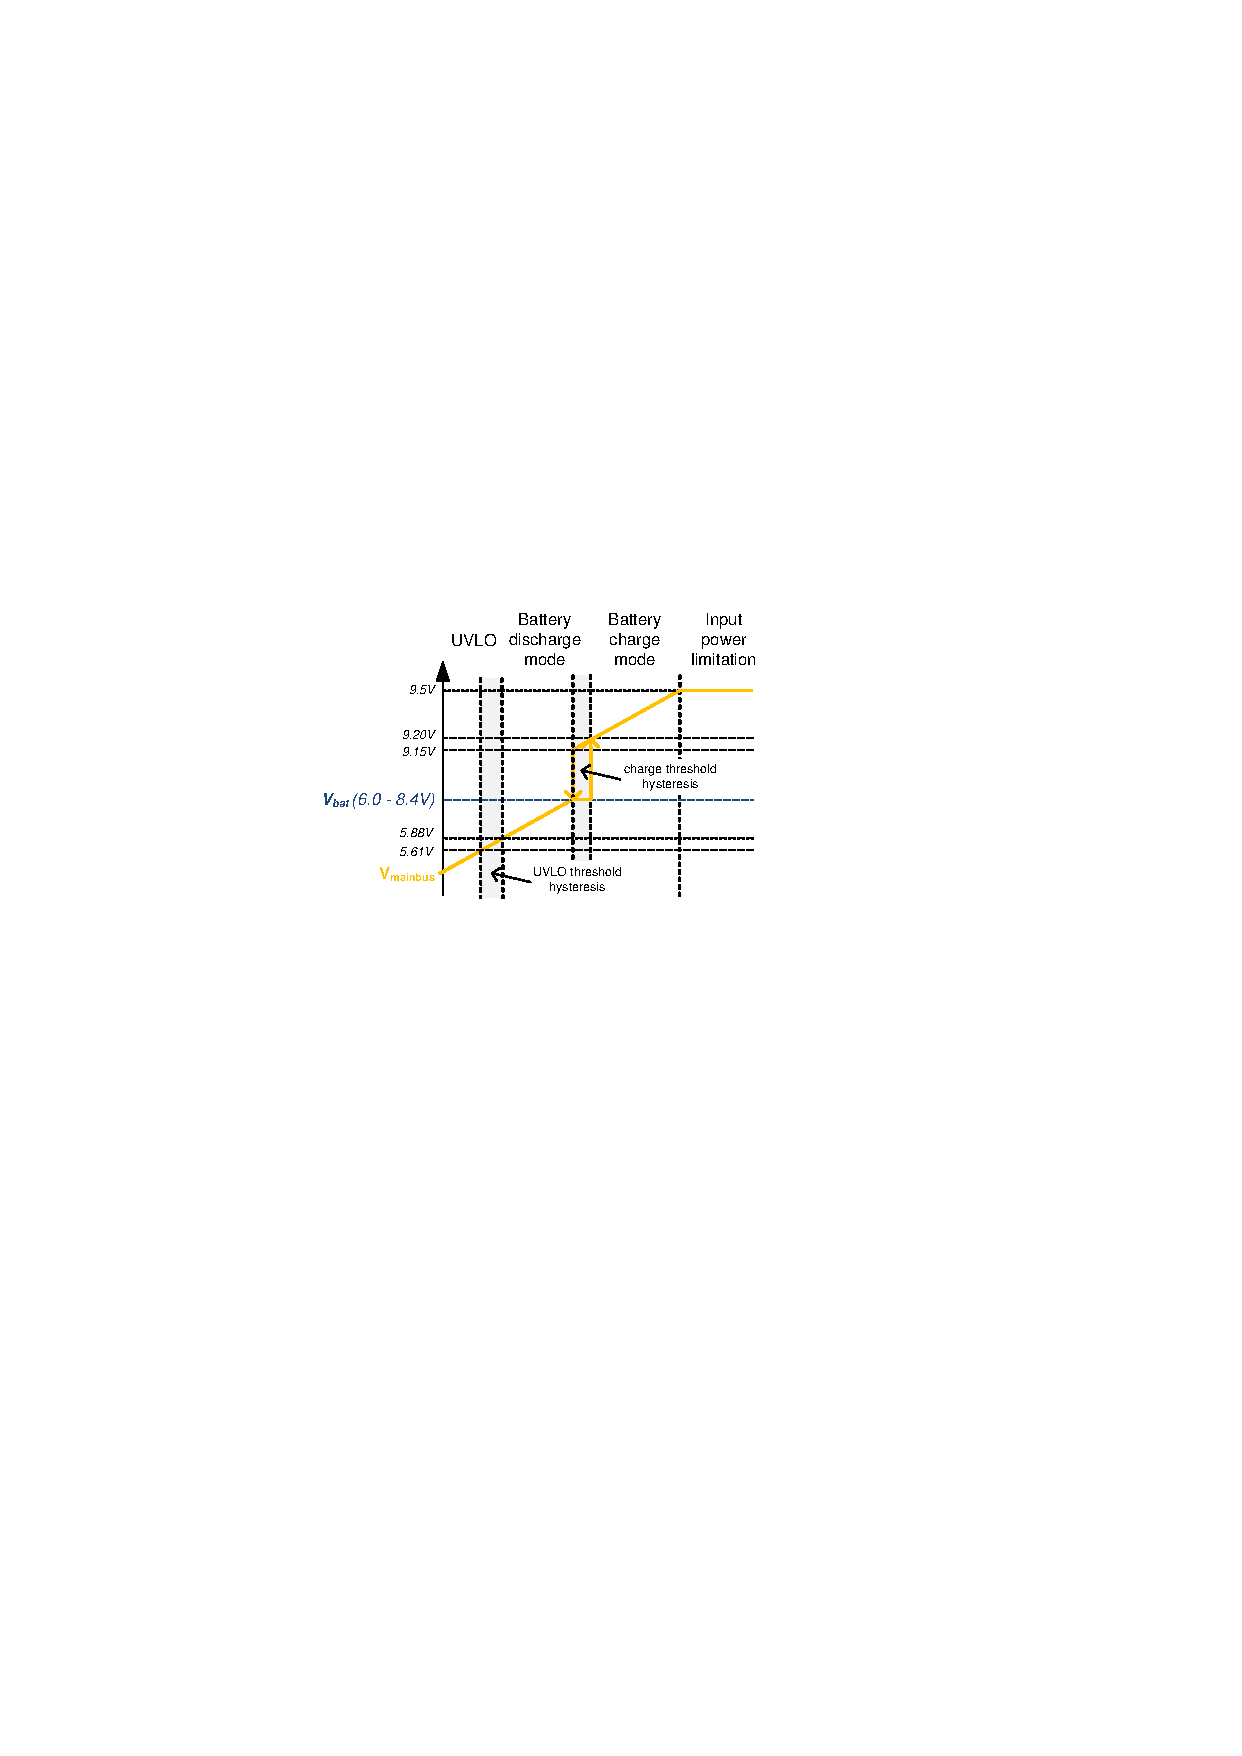
\includegraphics[width=0.8\textwidth]{figures/fig_CDR_SAR_ModeTransition}
\caption{Different SAR operation modes as function of mainbus voltage}
\label{fig:SAR_ModeTransition}
\end{figure}%
%
%
\subsection{3.3V and 5V Regulators}
To provide regulated $3.3\,V$ and $5\,V$ supplies for on-board logic circuits and payloads, a \textit{MIC29300-5} \ac{LDO} and a [3.3V regulator name] regulator are selected. Resettable $2\,A$ \ac{PTC} fuses are added to protect the loads from excessive currents and to protect the battery in case of a payload short-circuit failure.
%
\subsection{Complete Electrical Power System Diagram}
%
The complete \ac{EPS} diagram is shown in Figure \ref{fig:EPS_diagram_detailed}. Two $17\,A$ fuses are added in front of the motors to protect the battery from a motor short-circuit failure.
%
\begin{sidewaysfigure}
\centering
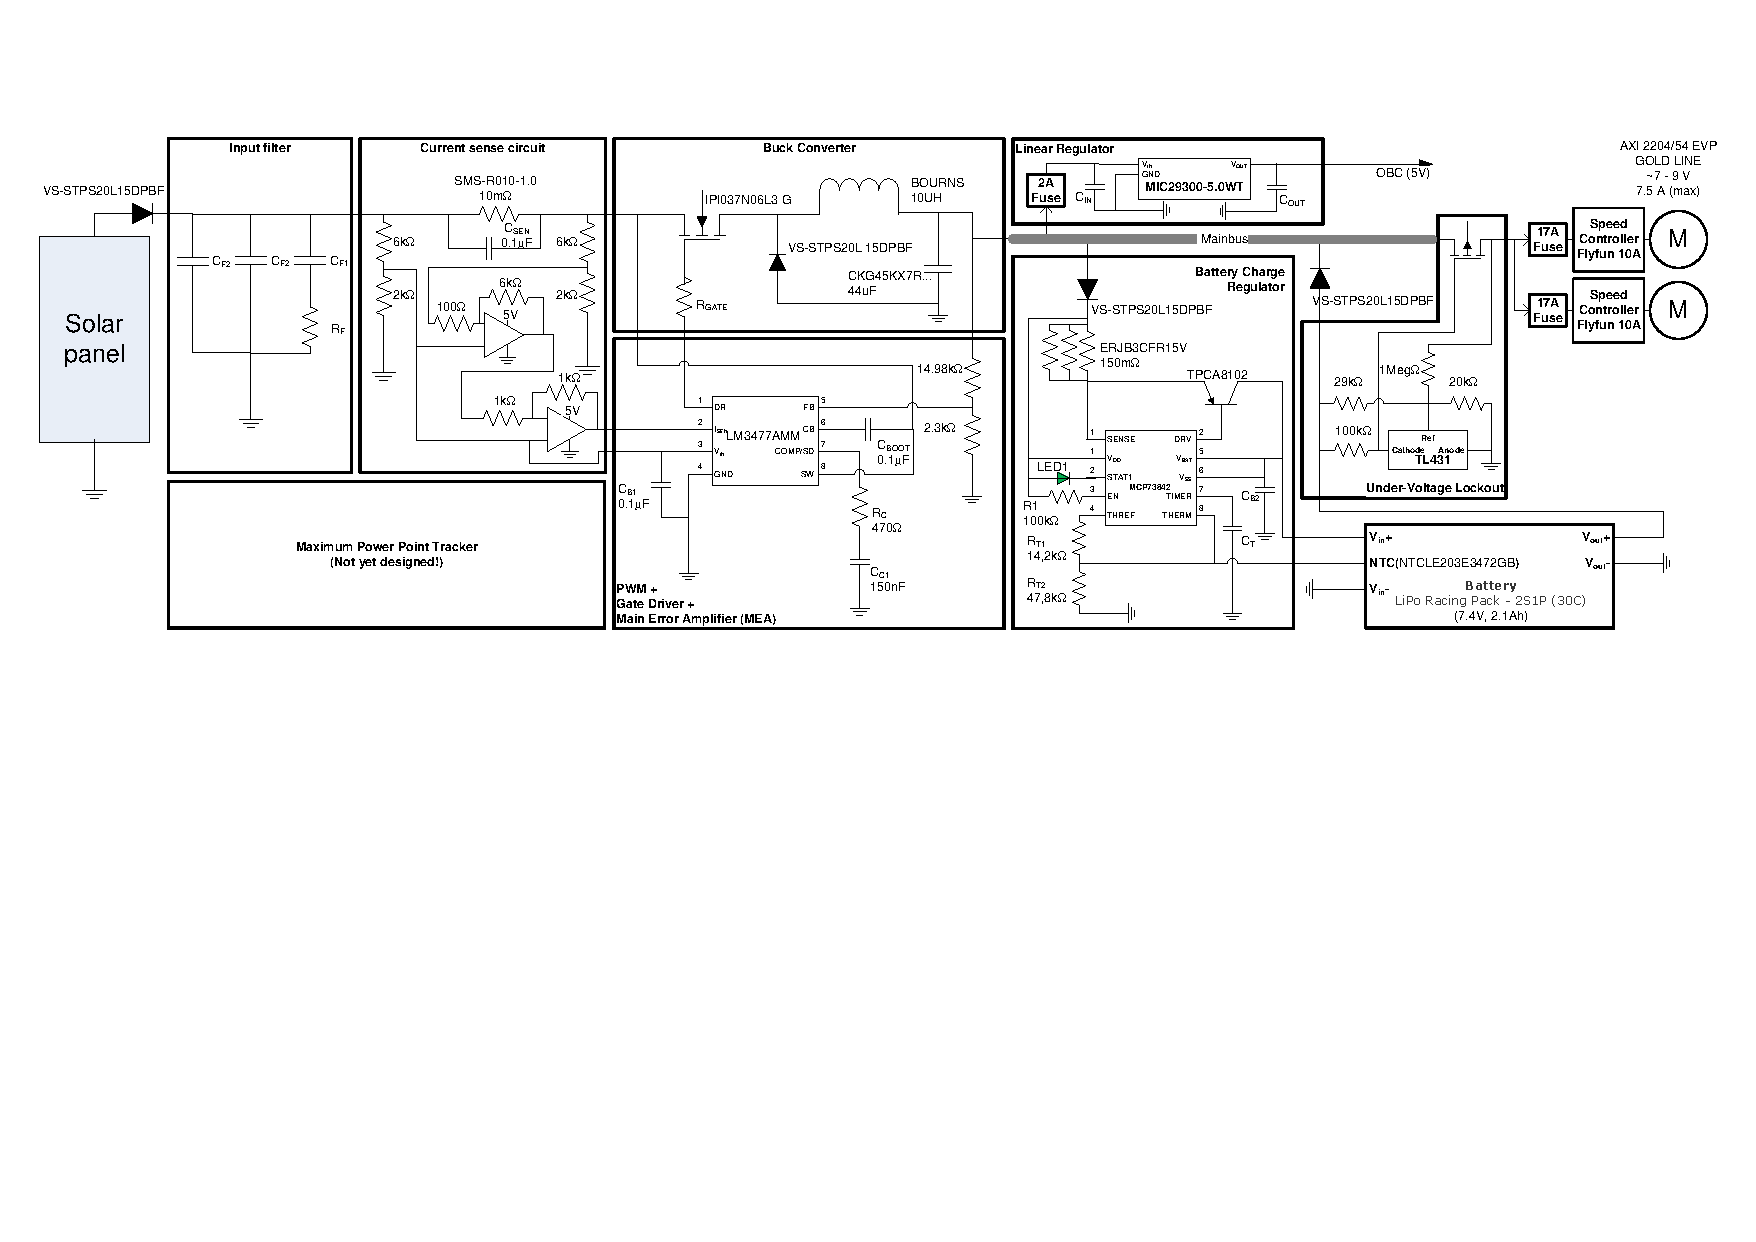
\includegraphics[width=\textwidth]{figures/fig_CDR_EPSdiagram_detailed}
\caption{EPS detailed block diagram}
\label{fig:EPS_diagram_detailed}
\end{sidewaysfigure}
%
\subsection{External Interfaces}
%
The external interfaces of the \ac{EPS} are listed in Table \ref{tab:external_interfaces_eps}.
%
\begin{table}[H]
\centering
\caption{EPS external interfaces}
\label{tab:external_interfaces_eps}
\begin{tabular}{p{0.25\textwidth}p{0.15\textwidth}p{0.5\textwidth}}
\hline
\textbf{External interface} & \textbf{Type} & \textbf{Implementation}\\
\hline
Solar cells mounting & Mechanical & Possibly using \ac{PSA} - \ac{TBD}.\\[2mm]
\rr Power electronics mounting & Mechanical & \rr Mounted on a \ac{PCB} which sits in the cargo bay, attached with screws.\tn[2mm]
Battery mounting & Mechanical & Mounted in cargo bay with strips or Velcro. Thermal insulation with Styrofoam or similar material should be added to protect against cold temperatures.\\[2mm]
\ac{EPS} telemetry & Electrical & Analog signals to microcontroller. Electrical connector interface still remains \ac{TBD}.\\[2mm]
\ac{EPS} telecommands & Electrical & \ac{TBD}\\[2mm]
Output voltages & Electrical & \rr $6.0-9.5\,V$ (un-regulated) and $5.0\,V$(regulated).\tn[2mm]
\hline
\end{tabular}
\end{table}
%
%
\subsection{Telemetry and Telecommands}
The suggested \ac{EPS} telemetries are listed in Table \ref{tab:Telemetry} and the suggested telecommands in Table \ref{tab:Telecommands}. Not all telemetries or telecommands are part of the initial \ac{EPS} design and will only be implemented if time and resources allow it.
\\
\\
The exact electrical configuration and interface connectors still remains to be designed.
%
\begin{table}[H]
\centering
\caption{\ac{EPS} telemetry}
\label{tab:Telemetry}
\begin{minipage}{\textwidth}
\begin{tabular}{|p{0.29\textwidth}p{0.13\textwidth}p{0.13\textwidth}p{0.35\textwidth}|}
\hline
\textbf{Telemetry} & \textbf{Data rate} & \textbf{Data size} & \textbf{Data range}\\
\hline
Battery voltage & Every 5 sec & 2 bytes & $5\,V$ to $9\,V$\\
\hline
Battery temperature & Every 5 sec & 2 bytes & $-25^{\circ}C$ to $+55^{\circ}C$\\
\hline
BCR status & Every 5 sec & 1 byte & \rr High($5\,V$), low($0\,V$) and $1\,Hz\;50\%$ duty cycle ripple\footnote{The different status indications are explained in the \ac{BCR} \ac{IC} datasheet}\tn
\hline
\ac{UVLO} status & Every 5 sec & 1 byte &  \rr $0\,V$(nominal operation), $5\,V$(under-voltage lock-out)\tn
\hline
Mainbus voltage & Every 5 sec & 2 bytes & $5\,V$ to $12\,V$\\
\hline
Solar array temperature & Every 5 sec & 2 bytes & $-35^{\circ}C$ to $75^{\circ}C$\\
\hline
Solar array voltage & Every 1 sec & 2 bytes & $10\,V$ to $20\,V$\\
\hline
\end{tabular}\par
\vspace{-0.75\skip\footins}
\renewcommand{\footnoterule}{}
\end{minipage}
\end{table}
%
\begin{table}[H]
\centering
\caption{EPS telecommands}
\label{tab:Telecommands}
%\begin{minipage}{\textwidth}
\begin{tabular}{|p{0.2\textwidth}p{0.25\textwidth}p{0.45\textwidth}|}
\hline
\textbf{Telecommand} & \textbf{Command signal} & \textbf{Description}\\
\hline
\rr Battery charge inhibit & logic low $(<0.8\,V)$ inhibits charging, logic high $(>1.4\,V)$ puts \ac{BCR} in normal mode & Battery charging can be remotely terminated in case of battery anomalies.\\
\hline
\rr Solar array voltage set & \ac{TBD} & When \ac{MPPT} is running, the solar array operating voltage can manually be set to mitigate any malfunction in the \ac{MPPT} algorithm.\\
\hline
\end{tabular}
\end{table}

\section{Test and Verification of Design}
\label{sec:test_verification}
This section describes the various design models used to develop the \ac{EPS} along with the expected functional test to be executed.
%
\subsection{Design Models}
%
\subsubsection{PSpice Simulations}
A transient PSpice simulation model of the whole \ac{EPS} is currently being implemented. The completed PSpice models are shown in Appendix \ref{app:EPS_PSpice}. These models will help in the design and testing of the regulator performance and system stability during transient loading as well as the interactions between the different circuits.
\\
\\
In the future, it is also desired to implement transient PSpice models for the solar array \cite{Castaner}, \ac{MPPTU}, battery \cite{gold}, motors and \ac{BCR}.
%
\subsubsection{Development Model}
An \ac{EPS} \ac{DM} is currently being built as seen in Figure \ref{fig:EPSprototype}. The prototype \ac{PCB} is realized using self-made "mini-mount" \ac{PCB} pads as shown in Appendix \ref{app:EPS_mini-mount}. These pads are attached, using a simple glue roller, on a complete copper ground plane. This design approach allows a compact layout which reduces parasitic effects. Also any \ac{IC} package can be supported and parts can easily be moved around when the design changes.
%
\begin{figure}[H]
\centering
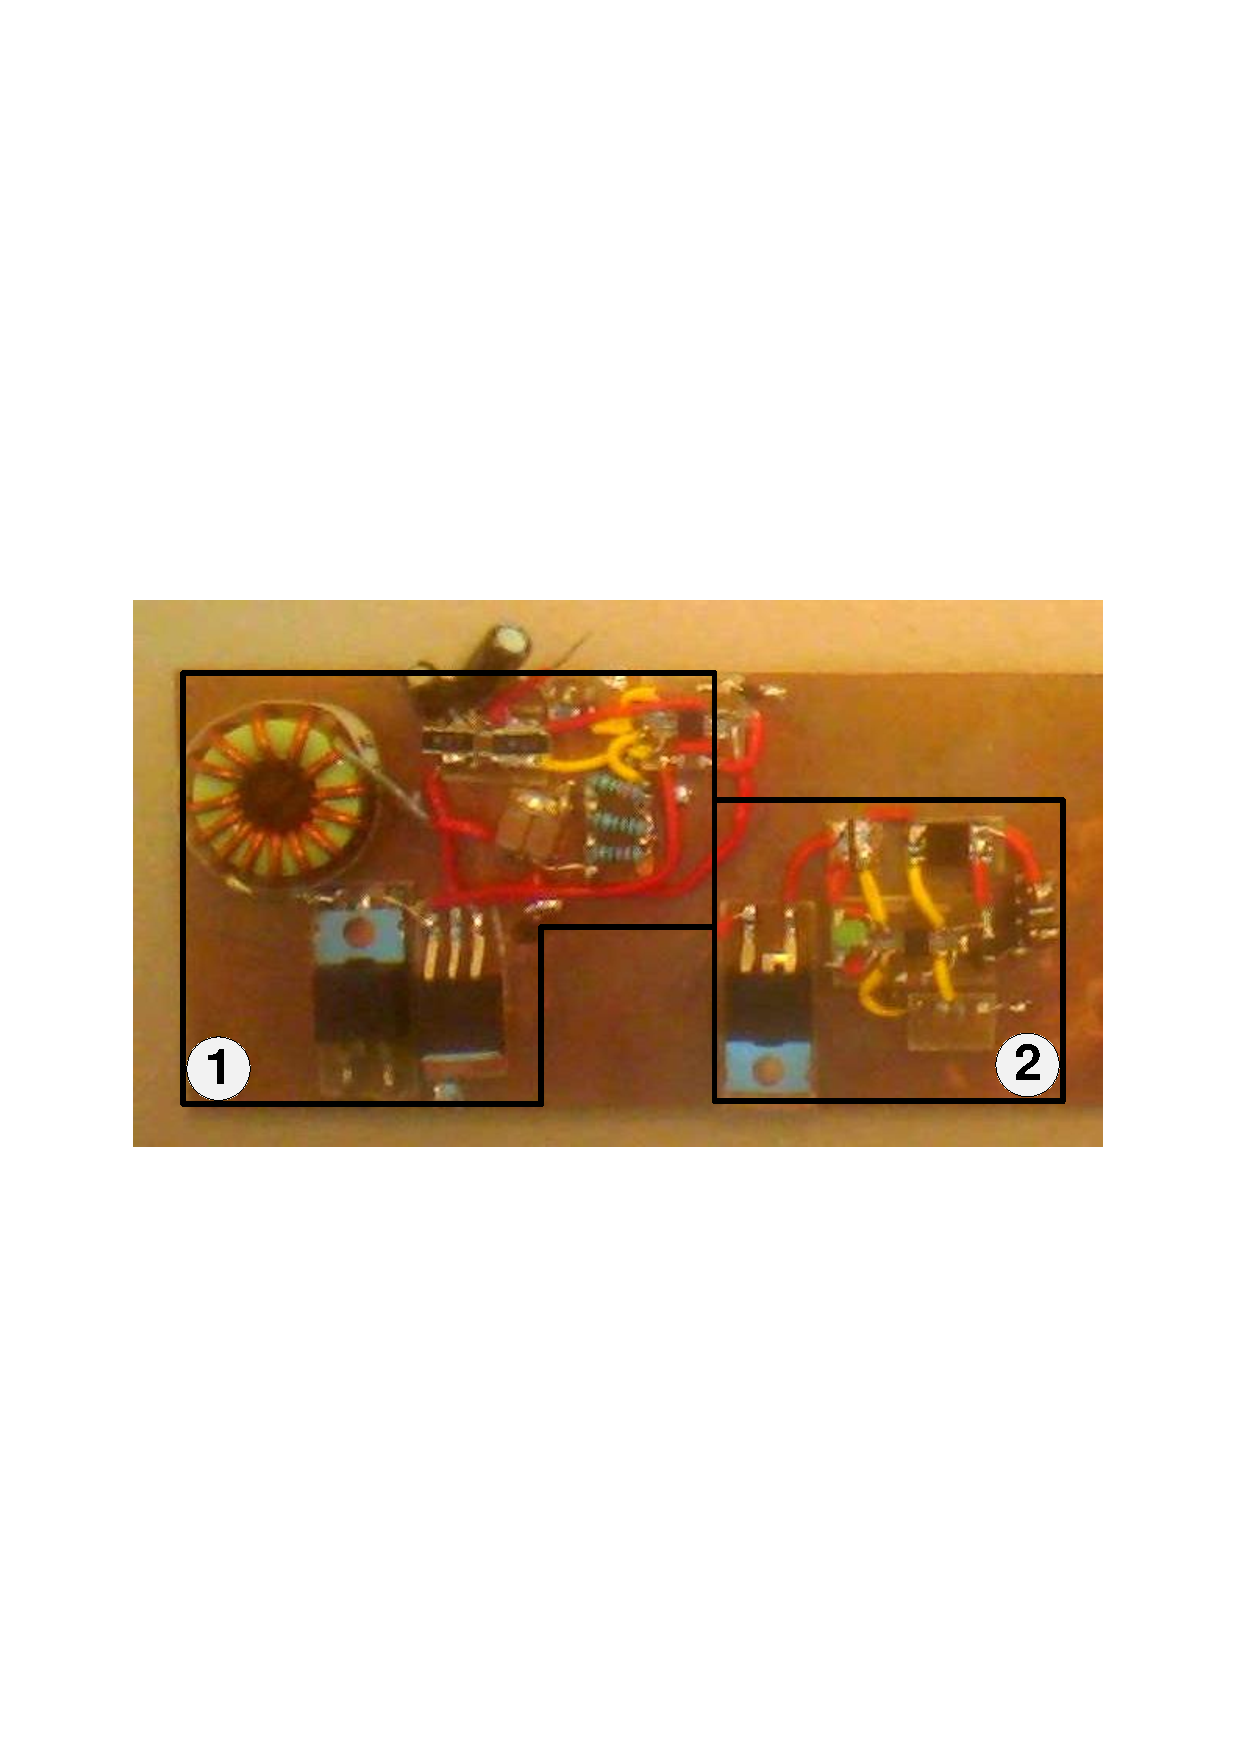
\includegraphics[width=0.8\textwidth]{figures/fig_CDR_EPSprototype}
\caption[EPS prototype]{EPS prototype - \textbf{1}: SAR, \textbf{2}: BCR}
\label{fig:EPSprototype}
\end{figure}
%
\subsubsection*{Development Model Status}
The \ac{SAR} is working but shows signs of \ac{CM} instability which is probably caused by the missing current sense amplifier circuit and input filter. Development progress is currently awaiting delivery of components. The \ac{BCR} is also working, however excessive heating of the \ac{MOSFET} was experienced. A new part rated for higher power dissipation has been selected and is currently awaiting delivery.
%
\subsubsection{Flight Model}
If time allows, a dedicated \ac{FM} will be built, using a custom designed \ac{PCB} schematic layout. An optimized \ac{PCB} layout will minimize the system mass and size while maximizing the efficiency and system robustness.
%
\subsection{Test Program}
\label{sec:eps_test_program}
Table \ref{tab:test_program} lists all necessary and desired test of the EPS. Priority "1" tests are all required while priority "2" tests will only be realized if time and resources allow it.
%
\begin{center}
\begin{longtable}[H]{p{0.15\textwidth}p{0.25\textwidth}p{0.45\textwidth}r}
\caption{EPS test program}\\
\label{tab:test_program}\\[-0.5cm]
\hline
\textbf{Subsystem} & \textbf{Condition/Mode} & \textbf{Test Description} & \textbf{Pri.}\\
\hline
\ac{SAR} & \rr Mainbus voltage limitation & \rr With more input power than load power, \ac{SAR} must be able to maintain a stable $9.5\,V$ output voltage also during transient loading. & 1\tn
- & \rr Maximum power handling & \rr With an input and load power slightly above the maximum expected solar array power, no \ac{SAR} components must overheat or otherwise malfunction. & 1 \tn
- & \ac{MPPT} & \ac{TBD}. & 2\\
- & Mode transitions & \rr \ac{SAR} must be able to change between \ac{MPPT}, battery charge and discharge mode without loosing mainbus voltage regulation or causing other malfunctions. & 2\tn
- & \rr Feedback loop stability & \rr Regulator bandwidth, gain- and phase margins should be measured with a network analyzer. & 2\tn
- & \ac{EMC} & Electromagnetic emissions should be measured with a spectrum analyzer, especially with regards to the telecommunication systems. & 2\\
\hline
\ac{BCR} & \rr \ac{CC} and trickle charging & \rr \ac{CC} charge at $2.4\,A$ and trickle charge mode entered when battery voltage reaches $8.4\,V$ should be verified. & 1\tn
- & \rr Charge inhibit at high/low temperatures & \rr While battery is charging, battery thermistor is heated/cooled in thermal oven/fridge to slightly above/below the specified temperature limits and charging should be terminated. & 1\tn
\hline
\ac{UVLO} & \rr Power cut-off and recovery & \rr Reducing input voltage below calculated threshold voltage should open switch and switch should close again when input voltage is increased above the threshold. & 1\tn
\hline
Battery & Dynamic model & Test approach is described in \cite{chen}. & 2\\
\hline
Solar cell & I-V specifications & \rr Short-circuit current, open-circuit voltage, current and voltage at the \ac{MPP} should be determined from an irradiance test. & 2\tn
- & \rr Temperature coefficients & \rr Solar cell temperature coefficients should be determined by measuring the I-V characteristics at different temperatures within the expected temperature interval. & 2\tn
\hline
Fuses & \rr Temperature variation & \rr The \ac{PTC} resettable fuses should be tested at nominal, minimum and maximum expected temperatures to verify acceptable functionality. & 1\tn
\hline
\end{longtable}
\end{center}
%

\section{Resources}
\label{sec:resources_scheduling}
%
%\subsection{Main Tasks}
%
%TBD...
%
%The main tasks, to implement the proposed \ac{EPS} design, are listed in table \ref{tab:main_tasks}.
%
%\begin{table}[H]
%\centering
%\caption{Main \ac{EPS} design and implementation tasks}
%\label{tab:main_tasks}
%\begin{minipage}{\textwidth}
%\centering
%\begin{tabular}{|p{0.05\textwidth}|p{0.5\textwidth}|p{0.15\textwidth}|p{0.2\textwidth}|}
%\hline
%\textbf{No.} & \textbf{Task} & \textbf{Duration [days]}\footnote{1 day = 8 effective working hours} & \textbf{Dependence (finish to start)}\\
%\hline
%1 & Design DC-DC regulator & 3 & - \\
%2 & PSpice regulator simulation & 5 & 1 \\
%3 & Order components and produce mini-mount patches\footnote{small pieces of PCB, with sticky bottom, very suitable for high frequency circuit prototyping} & 1 & 1, 2\\
%4 & Assemble solar cells & 3 & 1, 3\\
%5 & Design battery regulation and protection circuits & 3 & 1\\
%6 & Build and test battery circuits & 2 & 3, 5\\
%7 & Build prototype regulator (without MPPT) & 3 & 1, 3\\
%8 & Test prototype regulator (without MPPT) & 3 & 1, 2, 7\\
%9 & Design and build MPPT & 5 & 7\\
%10 & Test MPPT & 2 & 9\\
%11 & Design custom PCB layout & 2 & 1, 5, 9\\
%12 & Manufacture PCB and mount components & 3 & 11\\
%\hline
%\end{tabular}\par
%\vspace{-0.75\skip\footins}
%\renewcommand{\footnoterule}{}
%\end{minipage}
%\end{table}
%
\subsection{Parts List and Costs}
Table \ref{tab:parts_list} lists all ordered \ac{EPS} parts (including one order which is expected to be placed in the near future). The calculated costs do not include invoicing or shipping costs.
%
%
\begin{center}
\begin{longtable}[H]
{p{0.4\textwidth}p{0.25\textwidth}p{0.12\textwidth}rc}
\caption{EPS Parts list}\\
\label{tab:parts_list}\\[-0.5cm]
\hline
\textbf{Part} & \textbf{Part Name} & \textbf{Supplier} & \textbf{Cost\footnotemark[1]} & \textbf{Qty.}\\
\hline
\endhead
\footnotetext[1]{Unit price in SEK. Actual price may differ due to currency variations}
SAR current sense resistor & FCSL110R010FER & Farnell (US) & $31.52$ & 2\\
SAR power diode & MBR3050CT & Farnell & $9.24$ & 3\\
SAR power \ac{MOSFET} & IPI037N06L3 G & Farnell & $19.32$ & 4\\
SAR mainbus capacitor & CKG45NX5R1C226M & Farnell & $38.72$ & 4\\
PWM, MEA and \ac{MOSFET} driver & LM3477AMM & Farnell & $16.37$ & 5\\
SAR inductor & 2101-H-RC & Farnell (US) & $25.13$ & 2\\
\acp{PCB} & CIF - AA15 & Farnell & $67.42$ & 4\\
Battery(obsolete) & PA-L60 & Farnell & $294.28$ & 2\\
Battery & LiPo Racing Pack 2S1P & Ansmann & N/A\footnotemark[2] & 1\\
\footnotetext[2]{Part was supplied by previous Spacemasters}
Reverse protection diode & VS-STPS20L15DPBF & Farnell & $24.56$ & 6\\
BCR & MCP73842-840I/UN & Farnell & $13.61$ & 2\\
BCR Transistor(obsolete) & TPCA8102(TE12L,Q) & Farnell & $28.5$ & 2\\
\rr Current limit \ac{BJT} (obsolete) & 2STN2540 & Farnell & $7.84$ & 5\\
Current limit \ac{MOSFET} (obsolete) & IRLML6401PBF & Farnell & $6.41$ & 2\\
BCR current sense resistor & ERJB3CFR15V & Farnell & $1.97$ & 5\\
\rr Current limit sense resistor (obsolete) & ERJB2BFR33V & Farnell & $4.83$ & 5\\
\rr Current limit sense resistor 2 (obsolete) & ERJA1BJR27U & Farnell & $5.30$ & 5\\
Power limit \ac{BJT} (obsolete) & STN888 & Farnell & $5.49$ & 5\\
Solar cell & RC7.2-75(PSA) & Eco Power Shop & $230.08$ & 2\\
Solar cell (obsolete) & MC-SP0.8-NF-GCS & Farnell & $66.51$ & 2\\
\ac{LDO} regulator & MIC29300-5.0WT & Farnell & $74.85$ & 2\\
Current sense OpAmp & LTC6362CMS8\# PBF & Farnell & $32.31$ & 2\\
Thermistor & NTCLE203E3472GB0 & Farnell & $8.64$ & 5\\
Motor fuses & RGEF1000 & Farnell & $6.46$ & 5\\
\ac{LDO} regulator fuses & MC36248 & Farnell & $1.41$ & 5\\
\ac{BCR} \ac{MOSFET} & SUP75P03-07-E3 & Farnell & $31.51$ & 2\\
\ac{UVLO} linear shunt regulator & TL431AILPME3 & Farnell & $1.36$ & 5\\
\ac{UVLO} \ac{MOSFET} & SUP75P03-07-E3 & Farnell & $31.51$ & 2\\
\hline\hline
Total cost & & & 2707.6 & \\
\hline
\end{longtable}
\end{center}
%
%
\subsection{Electrical Ground Support Equipment}
The \ac{EGSE} in Table \ref{tab:EGSE} is mainly required for testing of the \ac{EPS}.
%
\begin{table}[H]
\centering
\caption{Required EGSE for EPS}
\label{tab:EGSE}
\begin{tabular}{|p{0.35\textwidth}p{0.55\textwidth}|}
\hline
\textbf{Instrument} & \textbf{Required Specifications}\\
\hline
Network Analyzer & Up to about $\sim 1\,MHz$\\
Spectrum Analyzer & \ac{TBD}\\
Power supply & $75\,W$ output power at $\sim 15\,V$\\
\rr Heating and cooling chamber(s) & $-20^{\circ}C$ to $+45^{\circ}C$ and allow wire interfacing through chamber\\
\hline
\end{tabular}
\end{table}
%
%
\subsection{Mechanical Ground Support Equipment}
The required \ac{MGSE} is mainly for \ac{PCB} manufacturing, i.e. UV light source, photo developing facility, etching facility, drills, cutters etc.
\chapter{Motor Control and Communication}
\label{chap:mcc}
The Motor Control and Communication subsystem is responsible for providing sufficient thrust to the airship for its movement and communication from ground. Two motors with propeller will be used for controlling the flight of the airship. Communication will be handled with commercial transmitters/receivers operating at 2.4GHz. 

\section{Functional and Technical Requirements}

Below are listed the primary functional requirements for the MCC:

\subsection{Functional Requirements}
%What function(s) does the subsystem have to fulfill?

\begin{itemize}
\item Reliable communication between ground controller (transmitter) \& airship (receiver)
\item Independent speed control for each of the motors and provision of sufficient thrust to the airship
\item Operation of the airship from ground 
\end{itemize}


\subsection{Technical Requirements}
%What technical requirements constrain the subsystem design? - e.g. mass, power, strength, stability etc.

MCC's technical requirements:

\begin{itemize}
\item Maximum power comsuption: 6.764W
\item Mass: 56g
\item Maximum cost: 2500 SEK
\item Input Voltage: 3.8 V
\item Thrust: 353.16 + 353.16 = 706.32 mN ( For Both Motor Propeller combo )
\item Transmission frequency: 2.4 GHz
\item Receiver channels: 6
\end{itemize}

As it was decided to use the blimp from ESRANGE instead of the structure that was supposed to be built by MSE, the whole system had to be re-designed. The main reasons were the dimensions of the blimp and the limitation on the total weight it is able to carry. This required for the MCC to use more powerful and efficient motors since the power system was affected as well, while the transmitter/receiver system remained unchanged.

Brushless motors were chosen as they are known to be more powerful and lighter at the same time ($26g$) and dimensions of $27,5\times 23 mm$. However this motors require a bit more current than the ones that were chosen originally. Therefore suitable ESC were chosen which are able to supply a maximum current of 10 $A$. 



\subsection{Expected Performance}
%What are the expected performances of the subsystem, as related to the requirements above? (maybe including some margins)

\begin{itemize}
\item Motors efficiency: 77 \% 
\item RPM (for each motor): 1400 RPM/V
\end{itemize}


\section{Design of the System}
%Explain the preliminary design including block diagrams, schematics, drawings, etc.

The functioning of the MCC subsystem is shown in the Figure \ref{fig:design_block}. The transceiver consists of 2.4 Ghz transmitter and receiver. The receiver gets the motor speed control commands to the ESC which in turn actuate the motor to the desired speed.

\begin{figure}[bht]
\centering
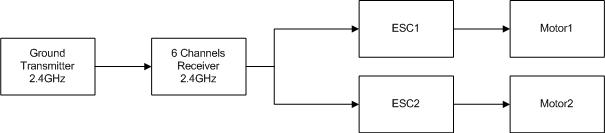
\includegraphics[scale=0.8]{figures/blockdiagram.jpg}
\caption{Block Diagram of the MCC Subsystem}
\label{fig:design_block}
\end{figure}

%\subsection{Software Structure}
%Explain the software structure (if relevant), including block diagrams, flowcharts, hierarchical structure, etc.

%some text...

%\begin{figure}[bht]
%\centering
%
\includegraphics[scale=0.5]{figures/Drawing1}
%\caption{Software structure}
%\label{fig:some_reference}
%\end{figure}


\subsection{Trade-Off Analysis of Concepts}
%Which design concepts are considered? - What are the advantages/disadvantages for each concept?

For the tranceiver system the available options are to use
\begin{itemize}
\item A 72 Mhz transceiver system that uses Amplitude/Frequency Modulation
\item A 2.4 Ghz tranceiver system that uses Spread Spectrum Technology
\end{itemize}

\begin{center}
\begin{table}[bht]
\rowcolors{3}{tableshade}{white}
\begin{tabular}{||l l l||}
\hline\hline
\textbf{Parameter:} &  \textbf{2.4 Ghz Tranceiver} & \textbf{72 Mhz Tranceiver}\\ 
\hline
Frequency Used & 2.4 Ghz & 72 Mhz \\
Crystal Used & No & Yes \\
Change in Frequency & On next power up & By changing the crystal \\
Ability to transmit through obstacles & Weak & Very Good\\
Band Width & Wide & Narrow\\
Date Rate & High & Low\\
Power Usage & Less & More\\
RF Noise Immunity & Very Good & Less \\
\hline
\end{tabular}
\caption{Trade off analysis}
\label{tab:TradeOff}
\end{table}
\end{center}

It is clear from the Table \ref{tab:TradeOff}, that a 2.4 GHz Tranceiver System is a clear winner for chosen application. The only disadvantage of using a 2.4 Ghz tranceiver system is that the receiver should have really good batteries and the voltage should be maintained at a paritcular level. The reason being that there are small processors in the transmitter and receiver that carry out many complex calculation every second without mistake. These processors require constant steady supply of current to work properly. If there is an interruption in the supply current of the receiver then there would be problems with the communication channel.

The speed of the motor can be controlled by the following methods:
\begin{itemize}
\item Use a commercial off the shelf Electronic Speed Controller(ESC) for each motor.
\item Build a Motor Speed Controller using a microprocessor.
\end{itemize}

The primamry advantage of using commercial off the shelf Electronic Speed Controller is the ease of use. This would reduce the development cycle to a large extent. The disadvantage of using it is no scalability i.e. function like autonomous control and telemetery and telecommanding are not possible.

\subsection{Argumentation for Chosen Concept(s)}
%Why is the chosen concept selected?

The 2.4 Ghz tranceiver system would be used for communication. The transceiver used 2.4 Ghz frequency band and uses the spread spectrum technology for transmission of signals. This helps in removing all interfering frequencies caused by other electronic equipments and this helps in having a better communication channel. The other major advantage of using this tranceiver using spread spectrum technology is that the communication channel would not be affected even by someone using the same frequency band.

Commercial off the shelf Electronic Speed Controllers would be used to control the speed of the motors because of time constraint in the project. If time permits it would be desirable to build a speed controller with the help of microprocessor.

\subsection{Feasibility Study of Concept(s)}
%How feasible is it to successfully implement the chosen concept? – Which potential issues/challenges might occur?

The important part in the communication part of the subsystem is deciding upon tranceiver system which would allow bidirectional control of the motor. Since tranceiver is commercial of the shelf, configuring it would be a short task.
Again in the case of motor speed control, choosing the correct ESC and motor combo is the most important task and given maximum time after which assembly is relatively easier and less time consuming.

\subsection{Telemetry and Telecommands}
%What telemetries/telecommands are required/useful for the subsystem? – What data rates/sizes are required?

If time permits, it would be desirable to have a microprocessor for telecommanding and telemetry  which is listed in Table \ref{tab:Telemetry}

\begin{table}[h]
\centering
\begin{tabular}{|l|l|l|}
\hline
\textbf{Telemetry} & \textbf{Data rate/frequency} & \textbf{Data size} \\
\hline
Battery voltage & Every 30 sec & 1 byte \\
\hline
Solar array temperature & Every 30 sec & 1 byte\\
\hline
Solar array voltage & Every 1 sec(MPPT Performance) & 2 bytes\\
\hline
Solar array temperature & Every 1 sec ( MPPT Performance & 2 bytes\\
\hline

\end{tabular}
\caption{Telemetry}
\label{tab:Telemetry}
\end{table}

\section{Electrical Circuits}

Explanation of all different circuits involved in the subsystem...
\chapter{Imaging and Tracking Payload Unit}
\label{chap:itpu}

General introduction to the subsystem...

\section{Functional and Technical Requirements}

Based on the PDR...

\section{?}

Again, no real suggestions here, but just describe your entire subsystem, including the software, autonomous functions, channel allocations, bit rate requirements, monitoring, etc.

\section{Electrical Circuits}

Explanation of all different circuits involved in the subsystem...
\chapter{Thermal Interfaces}
\label{chap:thermal}
%
%\section{Thermal Interfaces}
This chapter describes the \ac{U-SPACE} thermal requirements and design.
%
\section{Thermal Requirements}
The \ac{U-SPACE} systems are required to operate in the temperature range $-20^{\circ}\,C$ to $+45^{\circ}\,C$. The limits are based on weather data from Table \ref{tab:environment} including appropriate design margins. The high temperature limit also considers heat contribution from direct external sun exposure and internal power dissipation from the \ac{EPS}. Table \ref{tab:temp_critical_parts} lists temperature critical parts that are not rated for the full temperature range as given above.
%
\begin{table}[H]
\centering
\caption{Temperature critical parts}
\label{tab:temp_critical_parts}
\begin{minipage}{\textwidth}
\begin{tabular}{p{0.15\textwidth}p{0.2\textwidth}p{0.15\textwidth}p{0.15\textwidth}p{0.2\textwidth}}
\hline
\textbf{Part} & \textbf{Rating} & \textbf{Monitoring} & \textbf{Control} & \textbf{Protection}\\
\hline
BeagleBoard \ac{MCU} & $0^{\circ}\,C$ to $+85^{\circ}\,C$ & - & - & ?\\
\hline
\ac{EPS} Battery &  $+5^{\circ}\,C$ to $+40^{\circ}\,C$\footnote{Including $5^{\circ}\,C$ design safety margin} & External thermistor & - & Charge inhibit at low temperature.\\
\hline
\rr Current sense OpAmp & $0^{\circ}\,C$ to $+70^{\circ}\,C$ & - & - & -\tn
\hline
\end{tabular}\par
\vspace{-0.75\skip\footins}
\renewcommand{\footnoterule}{}
\end{minipage}
\end{table}
%
\section{Thermal Design}
From Table \ref{tab:temp_critical_parts} it is mainly the lower temperature limit which is of concern. Currently the \ac{U-SPACE} thermal design does not include temperature monitoring, except the battery, nor any temperature control. It will therefore not be possible to fly when the outdoor temperature falls much below $+5^{\circ}\,C$. This issue may be solved by insulating the cargo bay with Styrofoam or similar material. Internal dissipation from the \ac{EPS} and payloads will then increase the internal cargo bay temperature with respect to the outdoor temperature. Additional heaters may also be included in the design, however this will complicate the system and consume power which is already limited.\\[5mm]
Complete thermal analysis, insulation requirements and possible heater design still remains to be done.
%
\chapter{Electromagnetic Compatibility}
\label{chap:emc}
%
This chapter describes the \ac{U-SPACE} \ac{EMC}, \ac{EMI} susceptible parts and mitigation methods.\\[5mm]
%
%
For the \ac{U-SPACE} \ac{EMC} we have defined one mission critical circuit which is the motor control of the \ac{MCC} subsystem. Loss of motor control due to \ac{EMC} issues, could in the extreme case result in equipment damage. Two non-critical circuits have been identified: The ITPU sensors and the telemetry communication system. 
%
\section{Electromagnetic Interference Sources}
The identified main \ac{EMI} sources are:
%
\begin{itemize}
\item The \ac{EPS} \ac{SAR} - Radiated \ac{EMI} from power inductor and high AC-current loops. Conducted \ac{EMI} from power switches.
\item The two \ac{MCC} DC-motors - DC H-field from permanent magnet rotor and radiated \ac{EMI} when motors are running.
\item The \ac{MCC} motor power leads - Radiated \ac{EMI} from large AC-current loops (up to $\sim 7.5\,A$ per motor).
\end{itemize}
%
\section{Electromagnetic Interference Susceptibility}
%
Table \ref{tab:EMI_susceptibility_mitigation} lists the \ac{EMI} sensible parts which have been identified along with the applied mitigation method.
%
%
\begin{table}[H]
\centering
\caption{EMI susceptible parts and mitigation methods}
\label{tab:EMI_susceptibility_mitigation}
%\begin{minipage}{\textwidth}
\begin{tabular}{p{0.25\textwidth}p{0.25\textwidth}p{0.4\textwidth}}
\hline
\textbf{Susceptible part} & \textbf{Susceptibility type} & \textbf{Mitigation method}\\
\hline
\ac{ITPU} Magnetometer & DC H-fields &	Must be kept at minimum distance from DC-motors. Calibration might be necessary after \ac{ITPU} integration in complete \ac{U-SPACE} system.\\
\hline
\ac{ITPU} Sensors & \rr Radiated and conducted \ac{EMI} & Must be kept at minimum distance from \ac{EMI} radiation sources.\tn
\hline
\ac{MCC} motor communication & Radiated \ac{EMI} & Must be kept at minimum distance from \ac{EMI} radiation sources.\\
\hline
\rr \ac{MCC} telemetry communication & Radiated \ac{EMI} & Must be kept at minimum distance from \ac{EMI} radiation sources.\tn
\hline
\end{tabular}%\par
%\vspace{-0.75\skip\footins}
%\renewcommand{\footnoterule}{}
%\end{minipage}
\end{table}
%
%
\section{Electromagnetic Interference Mitigation Methods}
In \ac{U-SPACE}, the primary applied method for reducing \ac{EMI} related issues is to separate \ac{EMI} sources from \ac{EMI} susceptible parts be appropriate distances. It is also important to minimize the area of high AC-current loops. This can be achieved by proper \ac{PCB} layout of the \ac{SAR} and by keeping together and twisting the forward and return power leads to the DC-motors. A secondary method of mitigating radiated \ac{EMI} from the \ac{SAR} will be to apply shielding either around the complete circuit or only the power inductor. This will however increase the system mass and is therefore only a last-resort option.
%
%
\section{Electromagnetic Interference Tests}
\ac{EMI} tests for the \ac{EPS} were defined in Section \ref{sec:eps_test_program}. In general, susceptibility tests should be applied to the sensible parts defined in Table \ref{tab:EMI_susceptibility_mitigation}. When the \ac{EPS} \ac{SAR} and DC-motors are running at full power, no performance/communication degradation or glitches should be noticed, due to \ac{EMI}. Guides for \ac{EMI} emission measurements and susceptibility tests along with accepted limits are provided in \cite{ECSS_EMC}.
%
%

\chapter{Pyrotechnics Interface}
\label{chap:pyro}
%
%\section{Pyrotechnics Interface}
%
In order to achieve the functionality described in chapter \ref{chap:goals_constraints} there is no need for any form of pyrotechnics. The project does not require the release or deployment of other structures which could make use of pyrotechnics. Therefore pyrotechnics particulars are not discussed in this respect.
%
\section{Test and Verification of Design}
\label{sec:test_verification}
This section describes the various design models used to develop the \ac{EPS} along with the expected functional test to be executed.
%
\subsection{EPS Design Models}
%
\subsubsection{EPS PSpice Simulations}
A transient PSpice simulation model of the whole \ac{EPS} is currently being implemented. The completed PSpice models are shown in Appendix \ref{app:EPS_PSpice}. These will help in the design and testing of the regulator performance and system stability during transient loading as well as the interactions between the different circuits.

In future, it is desired also to implement transient PSpice models for the solar array\cite{Castaner}, \ac{MPPTU}, battery\cite{gold}, motors and \ac{BCR}.
%
\subsubsection{EPS Development Model}
An \ac{EPS} \ac{DM} is currently being build as seen in Figure \ref{fig:EPSprototype}. The prototype \ac{PCB} is realized using self-made "mini-mount" \ac{PCB} pads as shown in Appendix \ref{app:EPS_mini-mount}. These pads are attached, using a simple glue roller, on a complete copper ground plane. This design approach allows a compact layout which reduces parasitic effects. Also any \ac{IC} package can be supported and parts can easily be moved around if the design changes.
%
\begin{figure}[H]
\centering
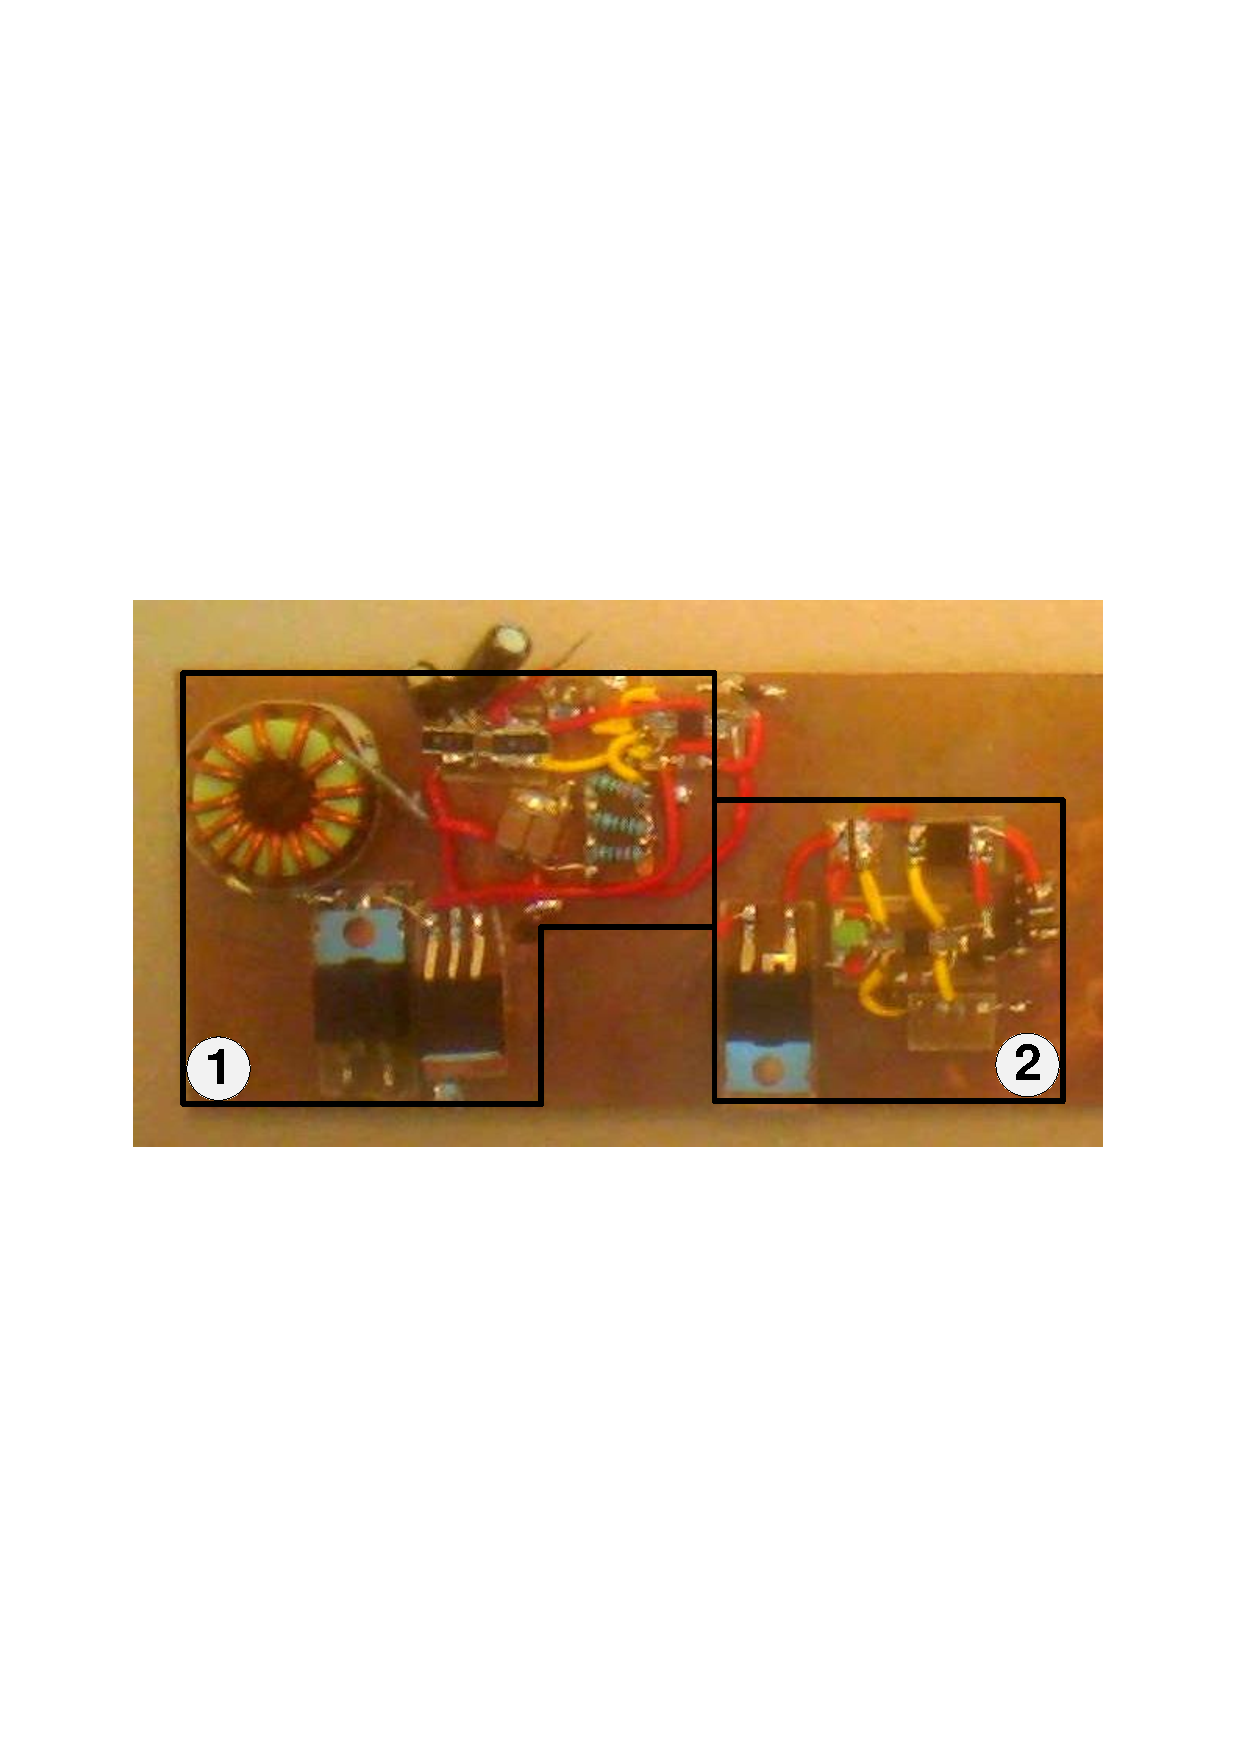
\includegraphics[width=0.8\textwidth]{figures/fig_CDR_EPSprototype}
\caption{\ac{EPS} prototype - \textbf{1}:\ac{SAR}, \textbf{2}:\ac{BCR}}
\label{fig:EPSprototype}
\end{figure}
%
\subsubsection*{Development Model Status}
The \ac{SAR} is working but shows signs of \ac{CM} instability which is expected to be caused by the missing current sense amplifier circuit and input filter. Development progress is currently awaiting delivery of components.

The \ac{BCR} is also working however excessive heating of the MOSFET was experienced. A new part rated for higher power dissipation has been selected and is currently awaiting delivery.
%
\subsubsection{EPS Flight Model}
If time allows, a dedicated \ac{FM} will be build, using a custom designed \ac{PCB} schematic layout. An optimized \ac{PCB} layout will minimize the system mass and size while maximizing the efficiency and system robustness.
%
\subsection{EPS Test Program}
Table \ref{tab:test_program} lists all necessary and desired test of the EPS. Priority "1" tests are all required while priority "2" tests will only be realized if time and resources allow it.
%
\begin{center}
\begin{longtable}[H]{p{0.15\textwidth}p{0.3\textwidth}p{0.45\textwidth}r}
\caption{EPS Test Program}\\
\label{tab:test_program}\\[-0.5cm]
\hline
\textbf{Subsystem} & \textbf{Condition/Mode} & \textbf{Test Description} & \textbf{Pri.}\\
\hline
\ac{SAR} & Mainbus voltage limitation & With more input power than load power, \ac{SAR} must be able to maintain a stable $9.5\,V$ output voltage also during transient loading & 1\\
- & Maximum power handling & With an input and load power slightly above the maximum expected solar array power, no \ac{SAR} components must overheat or otherwise malfunction & 1 \\
- & \ac{MPPT} & \ac{TBD} & 2\\
- & Mode transitions & \ac{SAR} must be able to change between \ac{MPPT}, battery charge and discharge mode without loosing mainbus voltage regulation or causing other malfunctions & 2\\
- & Feedback loop stability & Regulator bandwidth, gain- and phase margins should be measured with a Network Analyzer & 2\\
- & \ac{EMC} & Electromagnetic emissions should be measured with a Spectrum Analyzer, especially with concerns to the telecommunication systems & 2\\
\hline
\ac{BCR} & \ac{CC} and trickle charging & \ac{CC} charge at $2.4\,A$ and trickle charge mode entered when battery voltage reaches $8.4\,V$ should be verified & 1\\
- & Charge inhibit at high/low temperatures & While battery is charging, battery thermistor is heated/cooled in thermal oven/fridge to slightly above/below the specified temperature limits and charging should be terminated & 1\\
\hline
\ac{UVLO} & Power cut-off and recovery & Reducing input voltage below calculated threshold voltage should open switch and switch should close again when input voltage is increased above the threshold & 1\\
\hline
Battery & Dynamic model & Test approach is described in \cite{chen} & 2\\
\hline
Solar cell & I-V specifications & short-circuit current, open-circuit voltage, current and voltage at the \ac{MPP} should be determined from an irradiance test & 2\\
- & Temperature coefficients & Solar cell temperature coefficients should be determined be measuring the I-V characteristics at different temperatures within the expected temperature interval & 2\\
\hline
Fuses & Temperature variation & The \ac{PTC} resettable fuses should be tested at nominal, minimum and maximum expected temperatures to verify acceptable functionality & 1\\
\hline
\end{longtable}
\end{center}
%
\chapter{Ground Support Equipment}
\label{chap:ground_support}

\section{Electrical Ground Support Equipment (EGSE)}

The design, construction and test of a \ac{SPA} requires the use of extensive \ac{EGSE}, especially during test flights. The \ac{EGSE} can be divided into the ground station, the controller and some supplementary material.

\subsection{Concept}

The ground station of the \ac{U-SPACE} project is responsible for receiving data from the scientific payload and combining this data with images taken by the camera. This combination is then used to form aerial maps of the environment (see chapter \ref{chap:itpu}). It can also be used to track the airship with the help of the \ac{GPS} module and to visualize all data received from the airborne vehicle.
\\
\\
The controller is used to control the \ac{SPA} during flight (tests). It consists of a basic commercial transmitter/receiver  that allows a human ground-based pilot to remotely control the motors of the airship. More information can be found in chapter \ref{chap:mcc}.
\\
\\
The supplementary material of the \ac{EGSE} consists of a single power supply to charge the battery before flight. This allows the airship to start flying even without the presence of sunlight.

\subsection{Hardware Description}

For the ground station, the hardware is a desktop computer or laptop connected to a receiver. The basics of this system are described in chapter \ref{chap:itpu}. The pictures taken by the camera can be downloaded after flight (requiring a connection between the camera and the computer) or can be sent to the ground station when the \ac{SPA} is still airborne (via the same wireless connection used by the scientific payload data). The user is presented with visualizations of the scientific data as well as aerial maps constructed from the camera images and the scientific data (see chapter \ref{chap:itpu} for more information).
\\
\\
The hardware of the controller is basically a commercial remote controller capable of transmitting and receiving. By adjusting the controls the pilot is able to give more or less power to the motors mounted onto the airship. This is the principal means of forward propulsion. This controller system is described in more detail in chapter \ref{chap:mcc}.
\\
\\
Finally, the supplementary material consists of a commercial power supply that is able to charge the batteries of the \ac{EPS}. The characteristics of this battery are discussed in chapter \ref{chap:eps}.

\subsection{Software Description}

The supplementary power supply and the controller do not require any additional software. Only for the ground station additional software has to be developed, capable of reading the scientific payload data (received via the wireless connection) and visualizing this data for the user. In order to combine the aerial camera images and the scientific data a custom algorithm has to be written. This software is further described in chapter \ref{chap:itpu}.

\subsection{Compliance}

Both the ground station receiver and the controller transmitter/receiver have to comply with the Radio Regulations of the \ac{ITU} \cite{book:freqalloc}. As both hardware devices are commercial, no problems are expected in this respect.

\section{Mechanical Ground Support Equipment (MGSE)}

Apart from the \ac{EGSE}, also a certain amount of \ac{MGSE} is required for the success of the \ac{U-SPACE} project. First of all facilities at \ac{LTU} Rymdcampus, \ac{IRF} or Esrange have to be available during flight tests to enable on-site fuelling of the envelope with a suitable gas (see chapter \ref{chap:mse} for more details). These facilities include a large gas tank, valves and tubes to connect the tank to the envelope and also safety equipment to ensure that the entire procedure does not harm the persons involved.
\\
\\
Secondly an extensive safety system is necessary to prevent the airship from flying beyond the flight test perimeter in case of failures or unexpected weather conditions. This system should nevertheless allow the \ac{SPA} to move freely during all flight test procedures, without interfering with the normal operation of the airship. Possible implementations include a long rope tied to a fixed point or a cable firmly anchored to a movable object.
\chapter{Project Management}
\label{chap:project_management}

\section{Organisation and Responsibilities}

A project of the extent of the \ac{U-SPACE} project, even though it is a student project, requires clear agreements between the team members with with respect to responsibilities, work load and communication. Also the available support facilities and other practical issues have to be investigated beforehand.

\subsection{Key Personnel and Responsibilities}

Two important team members in the \ac{U-SPACE} project are the quality manager and the project manager. These managers were elected by the entire team. The quality manager, Morten Olsen, takes care of the technical side of the project. He is responsible for topics such as technical consistency between the different subsystems, follow-up of the progress of each subsystem and finally for guaranteeing the general technical quality of the project. The quality manager therefore gathers updated information from each subsystem, synthesizes this information and informs the project manager when problems arise. Currently Morten Olsen has also taken over the responsibilities of Dries Agten as project manager of the \ac{U-SPACE} project.
\\
\\
The project manager, Dries Agten, has responsibilities ranging from practical organisation over general communication to project documentation. The practical organisation includes the call for a weekly meeting, chairing this meeting, checking meeting reports, etc. With regards to communication the project manager is responsible both for internal and external communication. Therefore the project manager is in contact with the supervisors, Kjell Lundin (\ac{IRF}) and Alf Wikström (\ac{LTU}), to communicate the progress of the project and to have regular meetings to discuss this progress.  The internal communication topics range from calls for meetings to the passing-on of important information gained from the contact with the supervisors. Taking care of the project documentation means that the project manager is responsible for the design reviews, the meeting reports and other documentation that may be generated over the course of the project.

\subsection{Functional Organigram}

A functional organigram presenting the different subsystems (as defined in chapter \ref{chap:introduction}) and the associated team members is shown in figure ref{fig:obs}. This organigram is based on the background and expertise of the different team members (see table \ref{tab:backgrounds}), such that each team member is assigned a responsibility which he is able to handle.

\begin{figure}[bht]
\centering
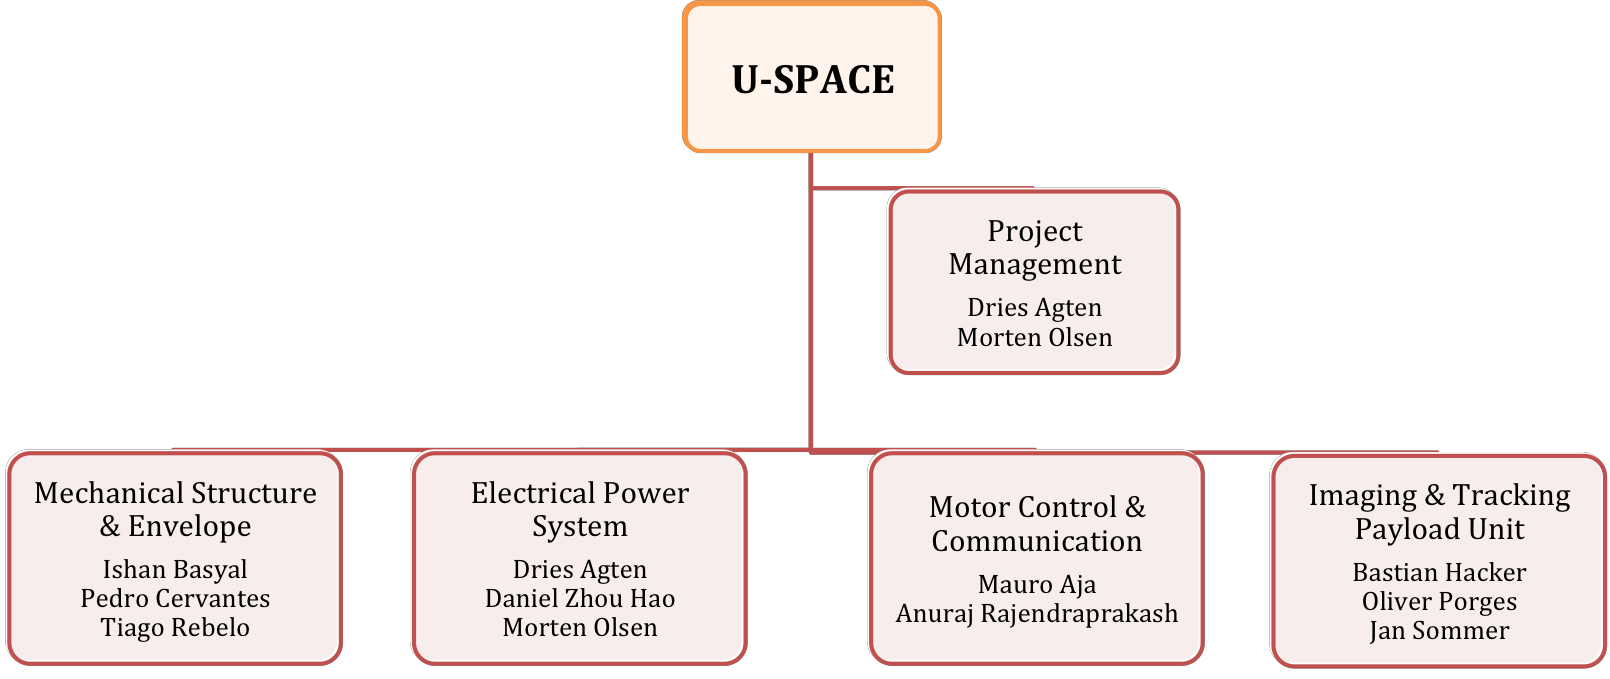
\includegraphics[width = \textwidth]{figures/obs.png} %scale=0.5
\caption{Functional organigram}
\label{fig:obs}
\end{figure}

\begin{table}[h]
\centering
\caption{Background of team members}
\begin{tabular}{l l}
\hline
\textbf{Name} & \textbf{Background} \\
\hline
Dries Agten & M.Sc. Eng. - Nanoscience \& Nanotechnology \\
Mauro Aja & B.Sc. Eng. - Electronic and Computer Engineering \\
Ishan Basyal & B.Sc. Earth and Space Sciences  \\
Pedro Cervantes & B.Sc. Eng. - Aeronautical Engineering \\
Bastian Hacker & B.Sc. Physics\\
Daniel Zhou Hao & B.Sc. Eng. - Aerospace Engineering\\
Morten Olsen & B.Sc. Eng. - Electrical Engineering \\
Oliver Porges & B.Sc. Cybernetics and Measurement  \\
Anuraj Rajendraprakash & B.Tech. Electronics Engineering \\
Tiago Rebelo & B.Sc. Eng. - Aeronautical Engineering \\
Jan Sommer & B.Sc. Computational Science \\
\hline
\end{tabular}
\label{tab:backgrounds}
\end{table}
%
\subsection{Support Facilities}
%
The support facilities of the \ac{U-SPACE} project are the responsibility of three organisations, each with a focus on a specific part of the project. The first organisation is \ac{LTU}, represented by Alf Wikström. As all team members are students from \ac{LTU}, this university is the principal support facility during the \ac{U-SPACE} project. Its responsibility is the practical, financial and also technical support of the team members. The practical support consists of providing tools and specific work spaces, such as mechanical workshops or electronics laboratories. Some other aspects are discussed in more detail in section \ref{sec:relation_support}.
\\
\\
The two other supporting organisations are \ac{IRF} and Esrange. \ac{IRF} is represented by Kjell Lundin, while the contacts with Esrange are the responsibility of Alf Wikström. These two support facilities provide technical assistance during the course of the project, consisting of guidance regarding the selection of the components, support during the fabrication procedures and recommendations regarding the test set-up.
%
\subsection{Transport}
%
The transportation of the prototype \ac{SPA} is an important topic in this project. Since the prototype will be built at the Rymdcampus of \ac{LTU} and since the test flight will most probably take place at Esrange, a secure transport procedure has to be developed. As the envelope is the property of Esrange (see chapter \ref{chap:mse}), the complete assembly of the airship will only take place at this location, which relieves the transport constraints. Most subsystem are limited in size and can easily be  transported in a normal passenger car. The only exception is the solar array and supporting mechanical structure which might be difficult to fit inside a car. A closed trailer or small truck might be needed for transportation of this.
%
%
\section{Relation With Support Facilities}
\label{sec:relation_support}
%
The support facilities mentioned in the previous section play an important role in the course of the \ac{U-SPACE} project. Their responsibilities are wide, ranging from reports over components to finances.
%
\subsection{Reporting and Monitoring}
%
During the entire project the team is monitored by the supervisors Kjell Lundin (\ac{IRF}) and Alf Wikström (\ac{LTU}). This monitoring task consists of controlling the budget, approving the ordering of components and evaluating the (technical) progress of the team at strategical points in time. Weekly meetings between the two supervisors and the two team managers are scheduled to identify, discuss and solve all issues that have come up since the last meeting. Apart from these weekly meetings, communication via email and telephone is used to keep the supervisors updated about the status of the project and to ask for assistance when needed.

\subsection{Reviews}
%
Three main reviews are planned for the \ac{U-SPACE} project:

\begin{itemize}
\item \acl{PDR}
\item \acl{CDR}
\item \acl{FRR}
\end{itemize}
%
The first two reviews are also the points in time when grades are connected to the work executed up to those points. Each review is briefly described below.
%
\subsubsection*{\acl{PDR}}
The \ac{PDR} was held and approved in early April 2012. With the help of five separate documents, the general project and the different subsystems were introduced to the supervisors, with a focus on the preliminary design concepts. The supervisors approval of the \ac{PDR} made the project budget available and allowed the first components to be ordered.
%
\subsubsection*{\acl{CDR}}
In the \ac{CDR}, which is the current document, the final designs of the subsystems are presented, together with some early verification and prototype results. An oral team presentation was held already in the middle of June 2012, before many team members had to leave Kiruna. The outcome of the \ac{CDR} is to ensure that the complete system design will meet the functional requirements from Section \ref{chap:goals_constraints} and the technical requirements stated for each subsystem. It must also show that all the system interfaces between different subsystems or the environment are compatible.
%
\subsubsection*{\acl{FRR}}
A third optional \ac{FRR} is also planned. This is to be held prior to flight, to ensure that all systems are fully functional and inter-compatible with each other and that all support equipment needed for a successful flight are available. This review is important since flight events at Esrange are expensive and the availability of the Esrange facilities and help from the staff is limited.
%
%
\subsection{Component Ordering}
%
The ordering of the components is the responsibility of \ac{LTU}, the organization that is also responsible for the project financing (see section \ref{sec:financing}). The members of the subsystems select the appropriate components and pass the order on to the project manager. He consults with the project supervisors and after approval the components are ordered, usually by Lars Jakobsson(LTU). Components are preferably ordered from inside Sweden, but international orders have also been possible.

\section{Financing}
\label{sec:financing}

The \ac{U-SPACE} project is financed by \ac{LTU}, the principal support facility. For each European team member, the team receives 2,000 SEK, amounting for a total budget of 14,000 SEK. This budget has to be used for the ordering of all components and for any other expenses that might arise during the course of the project (e.g. tools). An increase in the budget can be realized after an application procedure and approval by \ac{LTU}. As of this writing, the \ac{U-SPACE} project still has 4,824 SEK left of its initial budget. As was mentioned in Table \ref{tab:expected_performance}, a request for more funds for \ac{EPS} is under preparation.
%
%
\section{Schedule and Milestones}

Since the \ac{U-SPACE} project is a student project that has to be realized within a limited amount of time a tight schedule and a clear definition of important milestones are vital for the success of the project. The schedule has to updated regularly to reflect the current progress and/or delays of the project. The most recent schedule is shown in figure \ref{fig:schedule} below. All important milestones are indicated as well.

%\begin{figure}[htbp!]
%\centering
%\includegraphics[width=\textwidth]{figures/schedule.png}
%\caption{Current schedule and milestones.}
%\label{fig:schedule}
%\end{figure}

\textit{Morten, since I do not really have an idea about the status, I was hoping that you might be able to add this figure to the text. You know better what future milestones have to be realized as well...}

\section{Configuration Control}

Although the \ac{U-SPACE} project is limited in size, configuration control remains an important element of the success of the project. With four different subsystems and many different team members it is essential to have a common platform where design changes are listed, tracked and discussed. This is necessary to guarantee technical consistency and to avoid misunderstandings that may endanger the outcome of the project.
\\
\\
The main component of the \ac{U-SPACE} configuration control is a weekly meeting of all team members. An agenda is composed beforehand by the meeting chair, listing all important issues, both practical and technical, that have to be discussed during the meeting. A meeting secretary is responsible for producing minutes of the meeting. These minutes, together with the agendas, are accessible for the entire team by the use of Google Docs. Another minor component of the configuration control is the revision control system GitHub, which is mainly used to share the documents that make up the design review. It is also the place where the developed \ac{ITPU} code is made available to the relevant team members. For minor issues, emails to a common team email address are used.

\section{Deliverables}

The ultimate goal of the \ac{U-SPACE} project is to realize a functioning prototype of a \ac{SPA} capable of forward propulsion while supporting a scientific payload. Since this project is a student project under the supervision of \ac{LTU}, the final phases of the project also require the handing in of several deliverables.

\subsection{Hardware and Software}

The main deliverable is a functioning prototype of an \ac{SPA}, consisting of several separately developed subsystems (see chapters \ref{chap:mse} through \ref{chap:itpu}). Each subsystem should function on its own as well as in concurrence with the other subsystems. All necessary components have to be included when the subsystem is delivered.
\\
\\
Also the ground station is a deliverable, although it is mainly software-based. All code has to be delivered at the end of the project, together with comments that explain the code (see the following subsection). Also the code written for the airborne part of the \ac{ITPU} has to be included.

\subsection{Documentation}

The deliverable documentation first of all consists of both design reviews (\ac{PDR} and \ac{CDR}), which are documents that provide details on the functioning of each subsystem and on the general elements of the project. When available, all documents that were used during the development of a subsystem should be classified and stored for future use. This allows future team members to easily pick up the work where it was left by their predecessors.
\\
\\
Apart from these hardware-related documents, documentation regarding the developed software should also be delivered. This documentation mainly consists of comments on the code such that it may be understood and further developed by future team members.

\newpage
\printbibliography
\markboth{Bibliography}{Bibliography}
\addcontentsline{toc}{chapter}{\protect\numberline{}References}
\newgeometry{margin=1.5cm}
\pagestyle{plain}

\appendix

\chapter{Some Appendix}\label{app:SomeAppendix}
some text...

\chapter{Another Appendix}\label{app:AnotherAppendix}
some text...

\end{document}